% ===================== RESULTADOS =====================
\section{Resultados}
\label{sec:resultados}

Los resultados que se presentan a continuaci\'{o}n fueron extra\'{i}dos
program\'{a}ticamente del reporte de salida de CAESAR II del job
P2603-PR-SIM-023 (fecha de an\'{a}lisis: 09/10/2026). El modelo comprende
328 nodos evaluados.

% ─────────────────────────────────────────────────────────────────────────────
\subsection{Desplazamientos}

La Tabla~\ref{tab:desplaz-max} resume los desplazamientos m\'{a}ximos absolutos
por caso de carga, la Figura~\ref{fig:desplazamientos} muestra el perfil de
desplazamientos nodales del caso de operaci\'{o}n 1 (OPE) W+T1+P2 y la
Figura~\ref{fig:graf-desplazamiento} presenta la configuraci\'{o}n deformada del
modelo. El reporte del job no tabula los desplazamientos de los casos
sostenidos alternos 2 y 4 (Alt-SUS) W+P2, combinaciones sin gradiente
t\'{e}rmico cuyos movimientos quedan acotados por los de los casos de
operaci\'{o}n y sostenidos s\'{i} tabulados. Los desplazamientos son moderados:
el m\'{a}ximo corresponde a 34.5~\si{mm} en la componente $DZ$ del caso 8
(EXP, rango t\'{e}rmico de la condici\'{o}n $T_2$), con 26.2~\si{mm} en $DX$ y
4.2~\si{mm} en $DY$; en condici\'{o}n de operaci\'{o}n (caso 1) los m\'{a}ximos
son 10.1~\si{mm} en $DX$, 25.5~\si{mm} en $DY$ y 13.3~\si{mm} en $DZ$, valores
coherentes con el rango t\'{e}rmico ($\Delta T$~=~65~\si{\celsius}) y con la
longitud del colector de distribuci\'{o}n entre restricciones.

\begin{table}[htbp]
  \centering
  \small
  \caption{Desplazamientos máximos absolutos por caso de carga — línea SIM-023.}
  \label{tab:desplaz-max}
  \begin{tabular}{lrrr}
    \toprule
    Caso & max $|DX|$ (\si{mm}) & max $|DY|$ (\si{mm}) & max $|DZ|$ (\si{mm}) \\
    \midrule
    1 (OPE) & 10.106 & 25.486 & 13.291 \\
    3 (OPE) & 26.424 & 26.287 & 32.183 \\
    5 (SUS) & 17.131 & 25.338 & 13.636 \\
    6 (SUS) & 17.131 & 25.338 & 13.636 \\
    7 (EXP) & 9.833 & 0.826 & 4.972 \\
    8 (EXP) & 26.151 & 4.170 & 34.452 \\
    9 (EXP) & 16.318 & 3.652 & 32.061 \\
    \bottomrule
  \end{tabular}
\end{table}


\begin{figure}[htbp]
    \centering
    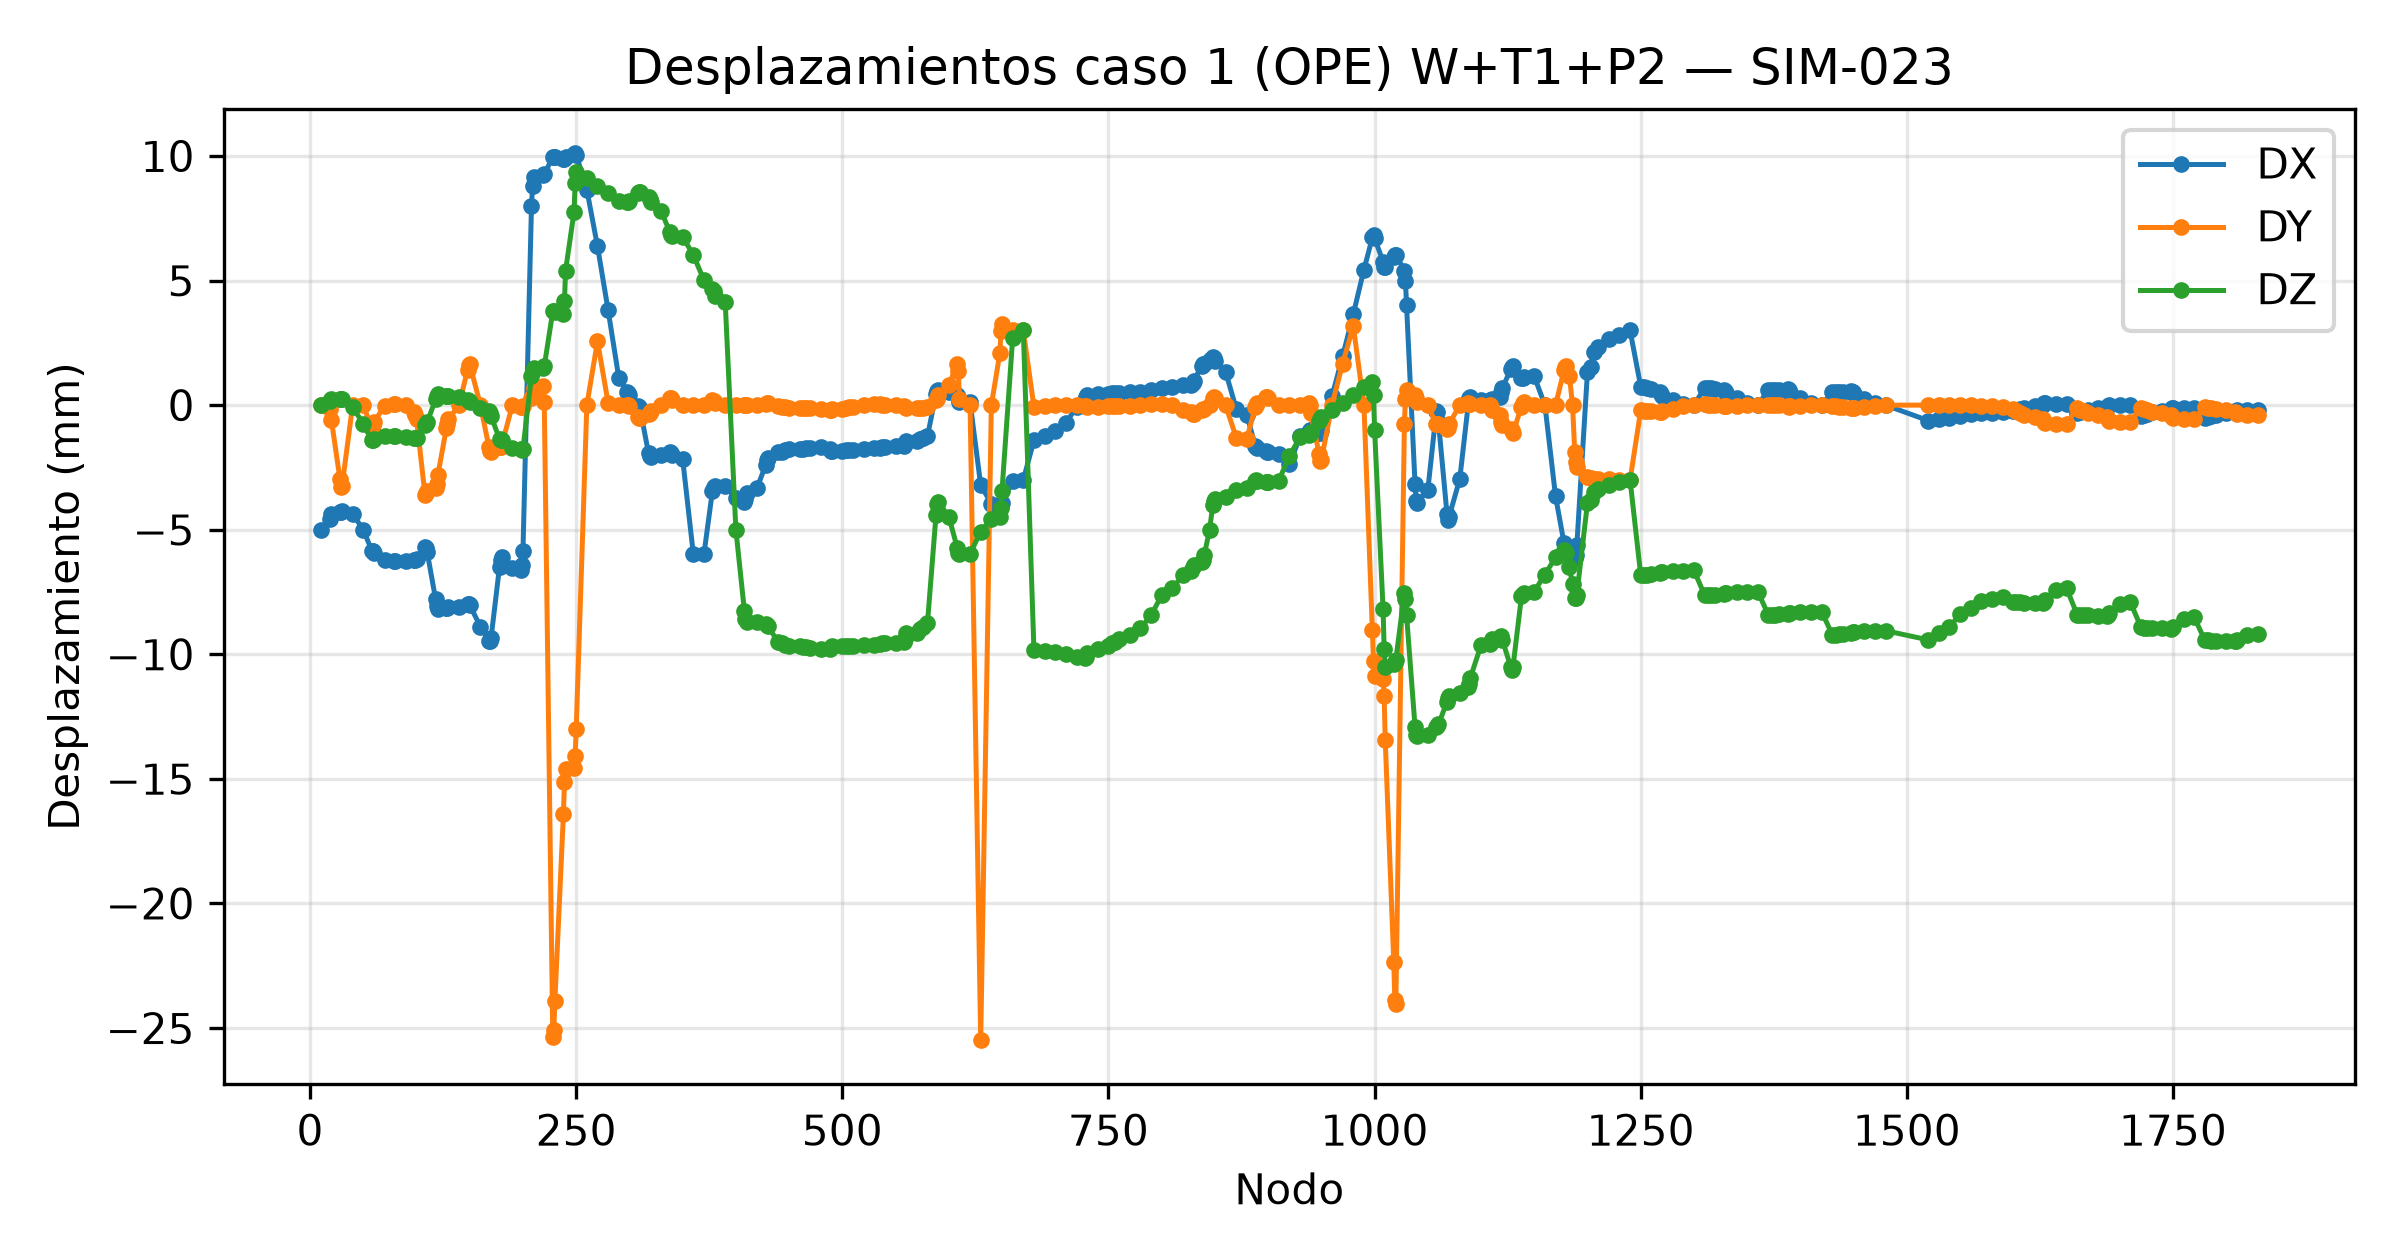
\includegraphics[width=0.85\textwidth]{assets/fig_desplazamientos.png}
    \caption{Perfil de desplazamientos nodales $DX$, $DY$ y $DZ$ en el caso 1 (OPE) W+T1+P2.}
    \label{fig:desplazamientos}
\end{figure}

\begin{figure}[htbp]
    \centering
    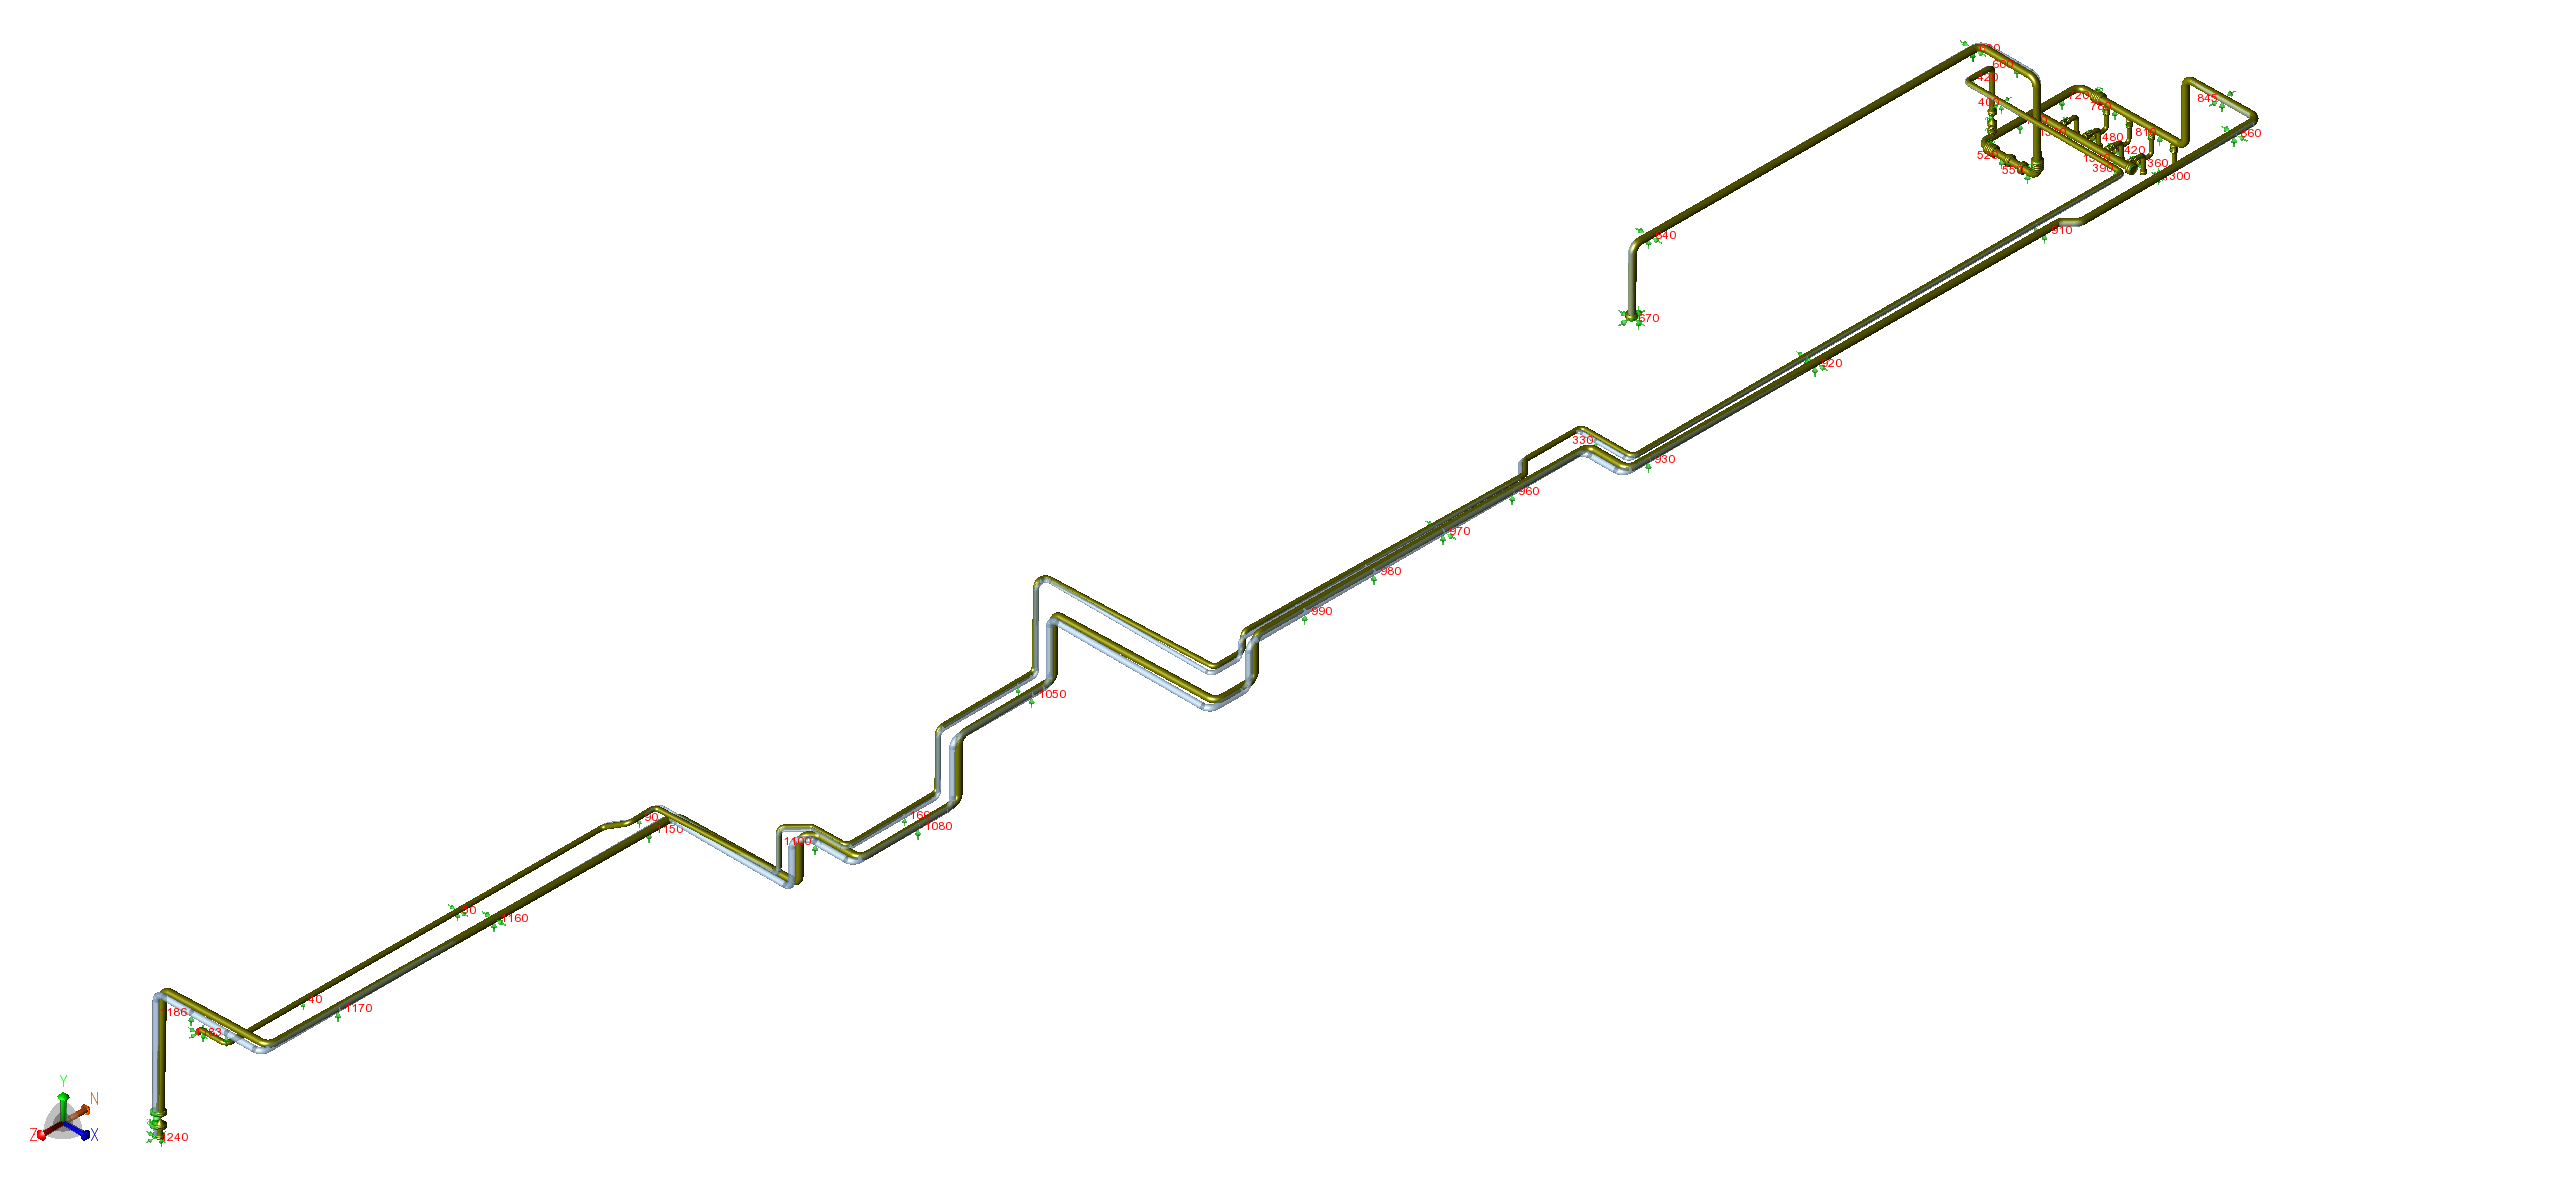
\includegraphics[width=0.85\textwidth]{assets/graf_desplazamiento.png}
    \caption{Configuraci\'{o}n deformada del modelo y distribuci\'{o}n de desplazamientos (CAESAR II, job P2603-PR-SIM-023).}
    \label{fig:graf-desplazamiento}
\end{figure}

% ─────────────────────────────────────────────────────────────────────────────
\subsection{Esfuerzos}

La Figura~\ref{fig:esfuerzos} presenta el perfil de esfuerzo de flexi\'{o}n
(\textit{bending}) por nodo para el caso cr\'{i}tico 2 (Alt-SUS) W+P2, la
Figura~\ref{fig:mapa-esfuerzos} muestra el mapa de esfuerzo de c\'{o}digo sobre
el modelo 3D para ese mismo caso, y la Tabla~\ref{tab:esfuerzos-critico}
consolida los valores de esfuerzo de c\'{o}digo, admisible y ratio de
utilizaci\'{o}n por nodo.

\begin{figure}[htbp]
    \centering
    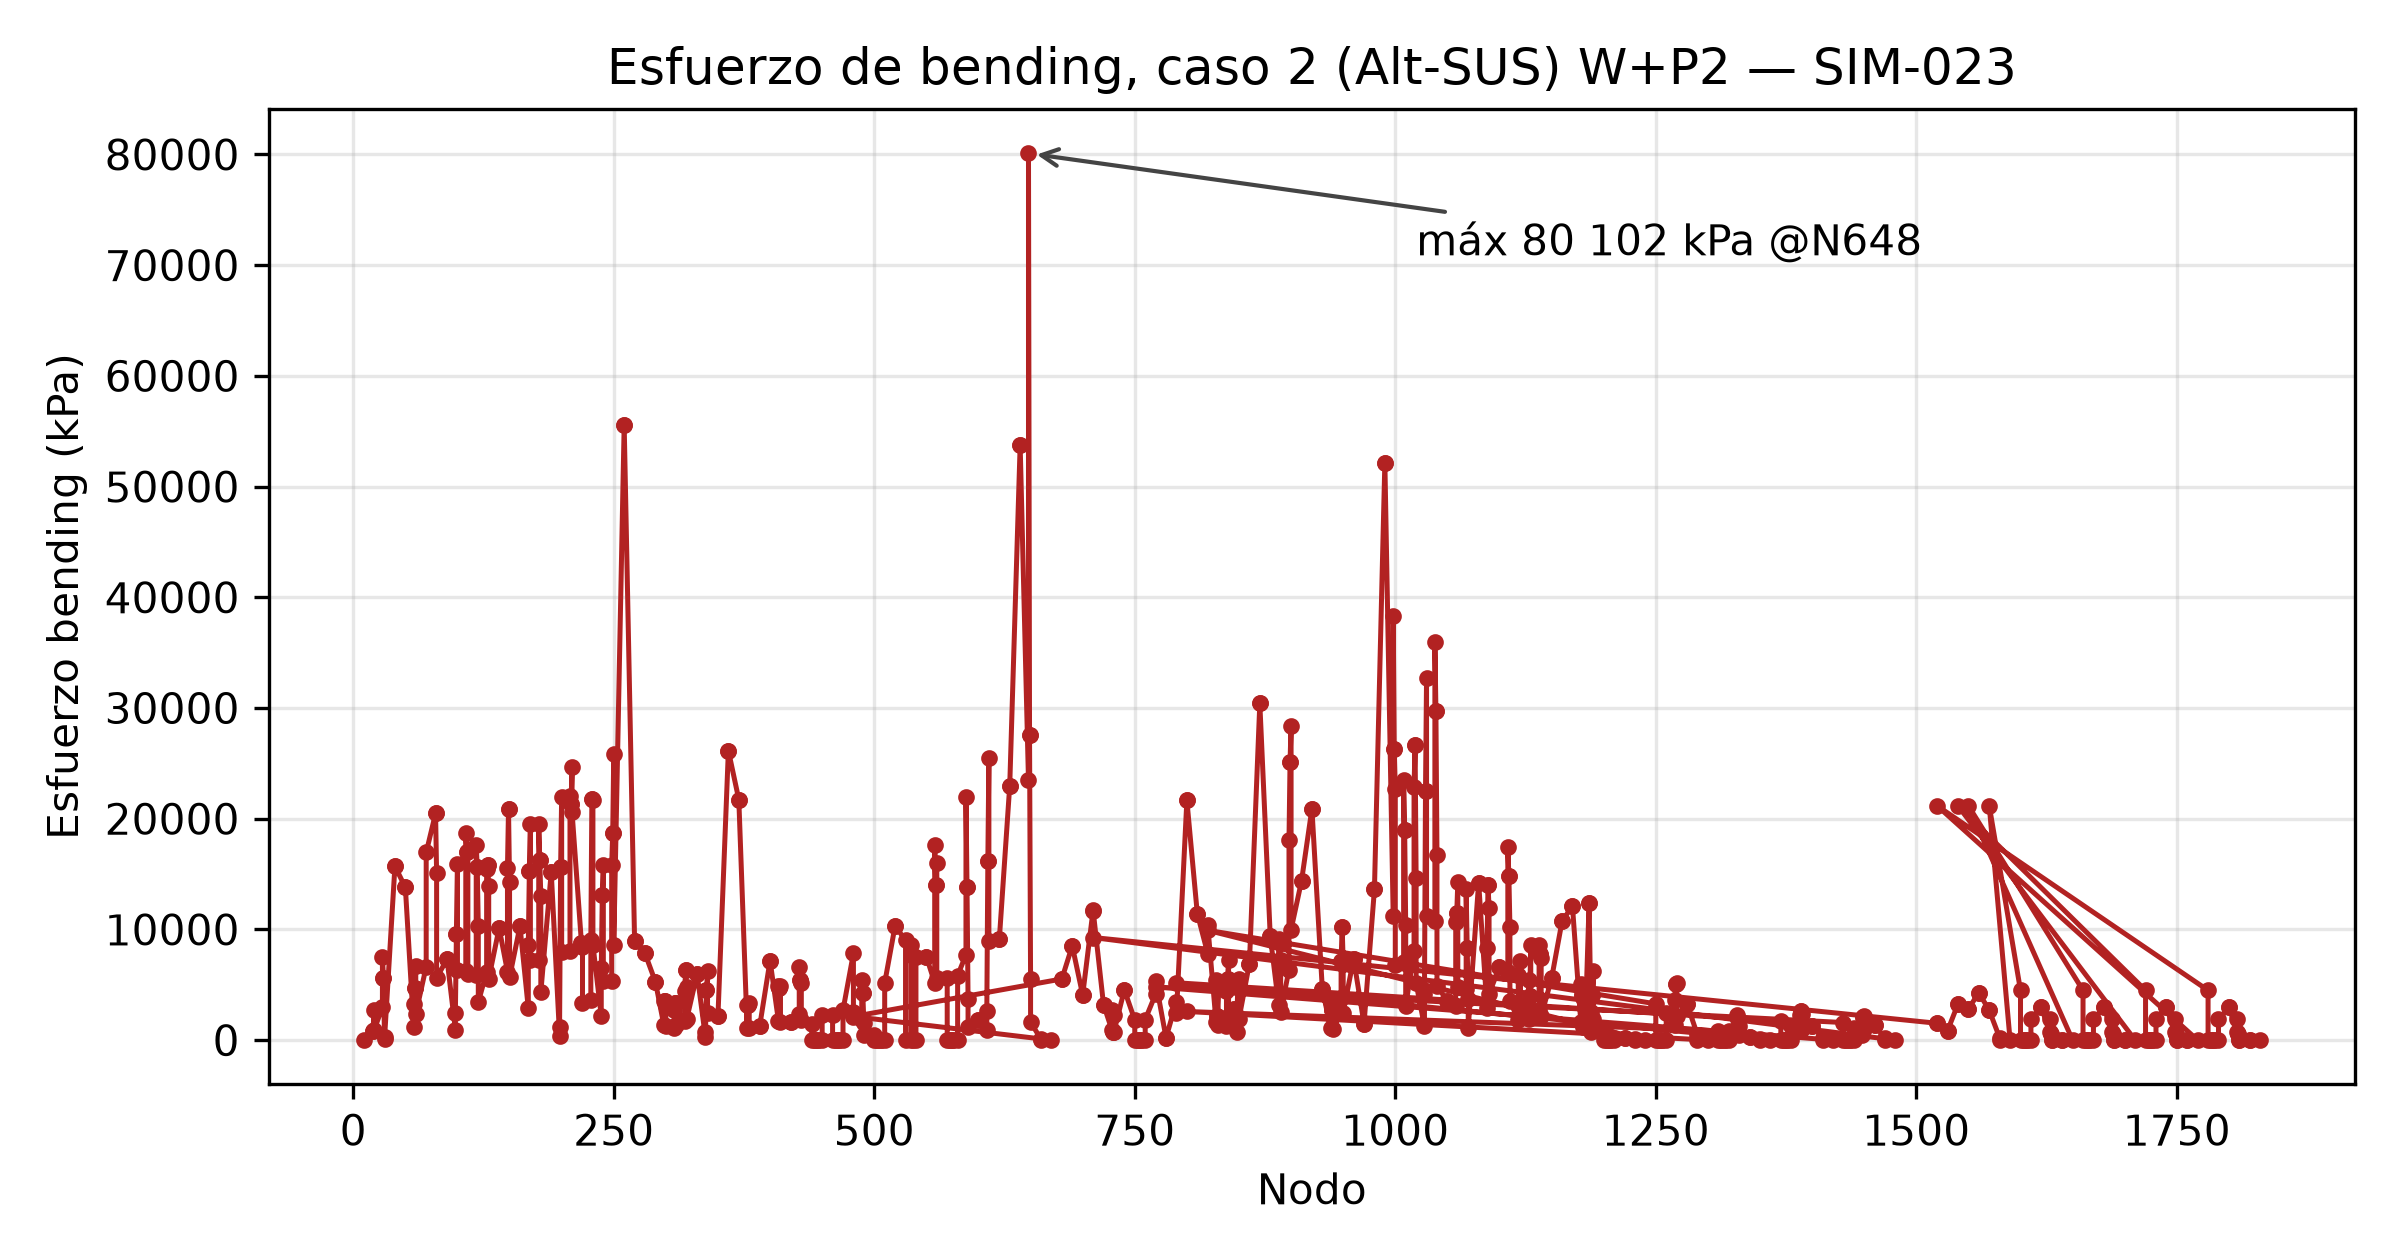
\includegraphics[width=0.85\textwidth]{assets/fig_esfuerzos.png}
    \caption{Perfil de esfuerzo de flexi\'{o}n por nodo, caso cr\'{i}tico 2 (Alt-SUS) W+P2. M\'{a}ximo: \num{80101.8}~\si{kPa} en el nodo 648.}
    \label{fig:esfuerzos}
\end{figure}

\begin{figure}[htbp]
    \centering
    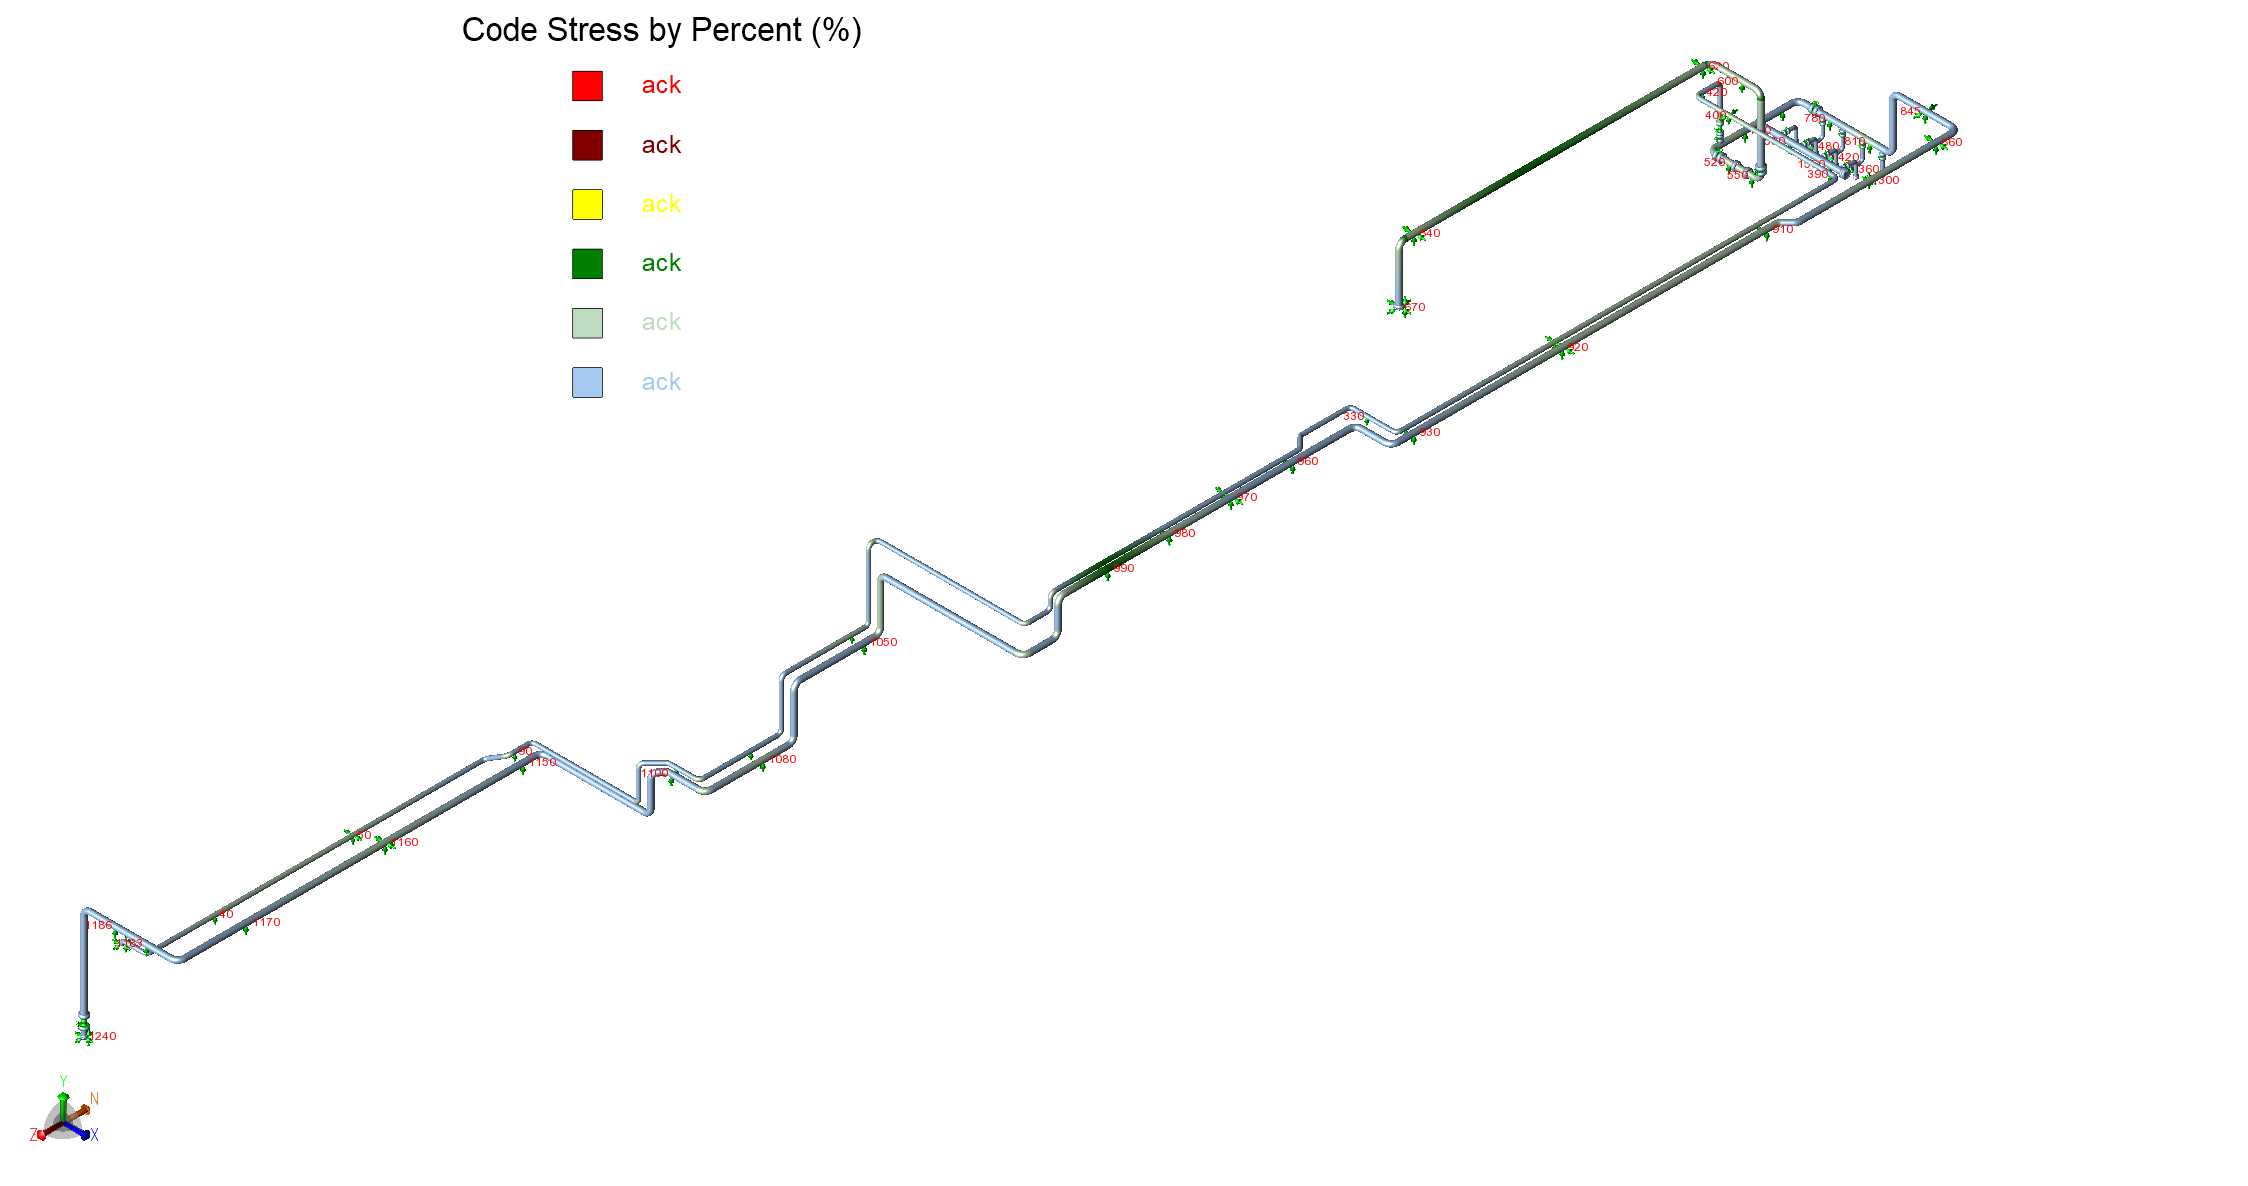
\includegraphics[width=0.85\textwidth]{assets/graf_stress_percent.png}
    \caption{Mapa de porcentaje de esfuerzo de c\'{o}digo (\textit{Code Stress by Percent}) sobre el modelo 3D, caso cr\'{i}tico 2 (Alt-SUS) W+P2 (CAESAR II, job P2603-PR-SIM-023). La escala de colores indica la relaci\'{o}n entre el esfuerzo de c\'{o}digo y el admisible en cada elemento.}
    \label{fig:mapa-esfuerzos}
\end{figure}

\begingroup
\footnotesize
\begin{longtable}{rrrrr}
  \caption{Esfuerzos por nodo, caso crítico 2 (Alt-SUS) W+P2 — línea SIM-023.}
  \label{tab:esfuerzos-critico} \\
    \toprule
    Nodo & Bending (\si{kPa}) & Code (\si{kPa}) & Allowable (\si{kPa}) & Ratio (\%) \\
    \midrule
  \endfirsthead
  \caption[]{Esfuerzos por nodo, caso crítico 2 (Alt-SUS) W+P2 — línea SIM-023 (continuación).} \\
    \toprule
    Nodo & Bending (\si{kPa}) & Code (\si{kPa}) & Allowable (\si{kPa}) & Ratio (\%) \\
    \midrule
  \endhead
    \midrule
    \multicolumn{5}{r}{(continúa en la página siguiente)} \\
  \endfoot
    \bottomrule
  \endlastfoot
    10 & \num{0.0} & \num{10529.9} & \num{115142.4} & 9.1 \\
    19 & \num{863.1} & \num{11245.7} & \num{115142.4} & 9.8 \\
    19 & \num{863.1} & \num{11245.7} & \num{115142.4} & 9.8 \\
    20 & \num{2698.6} & \num{12737.9} & \num{115142.4} & 11.1 \\
    20 & \num{895.7} & \num{11609.7} & \num{115142.4} & 10.1 \\
    28 & \num{2995.9} & \num{13709.9} & \num{115142.4} & 11.9 \\
    28 & \num{7521.9} & \num{16355.4} & \num{115142.4} & 14.2 \\
    29 & \num{5639.8} & \num{15101.2} & \num{115142.4} & 13.1 \\
    29 & \num{5639.8} & \num{15101.2} & \num{115142.4} & 13.1 \\
    30 & \num{294.3} & \num{11379.5} & \num{115142.4} & 9.9 \\
    30 & \num{111.8} & \num{11274.8} & \num{115142.4} & 9.8 \\
    40 & \num{15711.7} & \num{26611.0} & \num{115142.4} & 23.1 \\
    40 & \num{15711.7} & \num{26611.0} & \num{115142.4} & 23.1 \\
    50 & \num{13798.9} & \num{24712.8} & \num{115142.4} & 21.5 \\
    50 & \num{13798.9} & \num{24712.8} & \num{115142.4} & 21.5 \\
    58 & \num{1173.1} & \num{12297.2} & \num{115142.4} & 10.7 \\
    58 & \num{3266.6} & \num{13535.2} & \num{115142.4} & 11.8 \\
    59 & \num{4738.8} & \num{14745.4} & \num{115142.4} & 12.8 \\
    59 & \num{4738.8} & \num{14745.4} & \num{115142.4} & 12.8 \\
    60 & \num{6662.3} & \num{16058.3} & \num{115142.4} & 13.9 \\
    60 & \num{2376.4} & \num{13471.6} & \num{115142.4} & 11.7 \\
    70 & \num{6634.1} & \num{17733.4} & \num{115142.4} & 15.4 \\
    70 & \num{16950.9} & \num{23774.7} & \num{115142.4} & 20.6 \\
    79 & \num{20490.4} & \num{26485.7} & \num{115142.4} & 23.0 \\
    79 & \num{20490.4} & \num{26485.7} & \num{115142.4} & 23.0 \\
    80 & \num{15095.2} & \num{23648.0} & \num{115142.4} & 20.5 \\
    80 & \num{5615.1} & \num{18448.5} & \num{115142.4} & 16.0 \\
    90 & \num{7320.3} & \num{19973.3} & \num{115142.4} & 17.3 \\
    90 & \num{7320.3} & \num{19973.3} & \num{115142.4} & 17.3 \\
    98 & \num{939.5} & \num{14475.5} & \num{115142.4} & 12.6 \\
    98 & \num{2409.2} & \num{15182.3} & \num{115142.4} & 13.2 \\
    99 & \num{9573.2} & \num{19357.8} & \num{115142.4} & 16.8 \\
    99 & \num{9573.2} & \num{19357.8} & \num{115142.4} & 16.8 \\
    100 & \num{15952.4} & \num{22899.6} & \num{115142.4} & 19.9 \\
    100 & \num{6351.0} & \num{17359.0} & \num{115142.4} & 15.1 \\
    108 & \num{6217.4} & \num{17227.8} & \num{115142.4} & 15.0 \\
    108 & \num{18716.0} & \num{24953.6} & \num{115142.4} & 21.7 \\
    109 & \num{16955.2} & \num{23719.7} & \num{115142.4} & 20.6 \\
    109 & \num{16955.2} & \num{23719.7} & \num{115142.4} & 20.6 \\
    110 & \num{17129.6} & \num{23796.3} & \num{115142.4} & 20.7 \\
    110 & \num{5953.2} & \num{16904.2} & \num{115142.4} & 14.7 \\
    118 & \num{5885.6} & \num{16992.6} & \num{115142.4} & 14.8 \\
    118 & \num{17601.1} & \num{24305.9} & \num{115142.4} & 21.1 \\
    119 & \num{15599.5} & \num{22706.4} & \num{115142.4} & 19.7 \\
    119 & \num{15599.6} & \num{22706.4} & \num{115142.4} & 19.7 \\
    120 & \num{10328.4} & \num{18501.5} & \num{115142.4} & 16.1 \\
    120 & \num{3437.9} & \num{14206.8} & \num{115142.4} & 12.3 \\
    128 & \num{6141.1} & \num{16900.6} & \num{115142.4} & 14.7 \\
    128 & \num{15437.2} & \num{22325.4} & \num{115142.4} & 19.4 \\
    129 & \num{15846.1} & \num{22905.3} & \num{115142.4} & 19.9 \\
    129 & \num{15846.1} & \num{22905.3} & \num{115142.4} & 19.9 \\
    130 & \num{13916.2} & \num{22011.4} & \num{115142.4} & 19.1 \\
    130 & \num{5534.3} & \num{17354.2} & \num{115142.4} & 15.1 \\
    140 & \num{10131.0} & \num{21717.4} & \num{115142.4} & 18.9 \\
    140 & \num{10131.0} & \num{21717.4} & \num{115142.4} & 18.9 \\
    148 & \num{6198.1} & \num{17977.2} & \num{115142.4} & 15.6 \\
    148 & \num{15584.1} & \num{23215.8} & \num{115142.4} & 20.2 \\
    149 & \num{20901.4} & \num{26386.5} & \num{115142.4} & 22.9 \\
    149 & \num{20901.4} & \num{26386.5} & \num{115142.4} & 22.9 \\
    150 & \num{14257.7} & \num{22139.5} & \num{115142.4} & 19.2 \\
    150 & \num{5669.0} & \num{17329.8} & \num{115142.4} & 15.1 \\
    160 & \num{10290.0} & \num{21749.9} & \num{115142.4} & 18.9 \\
    160 & \num{10290.0} & \num{21749.9} & \num{115142.4} & 18.9 \\
    168 & \num{2861.8} & \num{14705.0} & \num{115142.4} & 12.8 \\
    168 & \num{8600.7} & \num{18070.2} & \num{115142.4} & 15.7 \\
    169 & \num{15279.2} & \num{22380.4} & \num{115142.4} & 19.4 \\
    169 & \num{15279.2} & \num{22380.4} & \num{115142.4} & 19.4 \\
    170 & \num{19528.0} & \num{25099.6} & \num{115142.4} & 21.8 \\
    170 & \num{7199.0} & \num{17653.7} & \num{115142.4} & 15.3 \\
    178 & \num{7220.2} & \num{17919.6} & \num{115142.4} & 15.6 \\
    178 & \num{19533.4} & \num{25348.4} & \num{115142.4} & 22.0 \\
    179 & \num{16288.7} & \num{23332.9} & \num{115142.4} & 20.3 \\
    179 & \num{16288.7} & \num{23332.9} & \num{115142.4} & 20.3 \\
    180 & \num{13025.3} & \num{21273.4} & \num{115142.4} & 18.5 \\
    180 & \num{4327.6} & \num{16102.4} & \num{115142.4} & 14.0 \\
    190 & \num{15182.3} & \num{26525.2} & \num{115142.4} & 23.0 \\
    190 & \num{15182.3} & \num{26525.2} & \num{115142.4} & 23.0 \\
    198 & \num{410.0} & \num{12522.2} & \num{115142.4} & 10.9 \\
    198 & \num{1193.3} & \num{12954.8} & \num{115142.4} & 11.3 \\
    199 & \num{15619.3} & \num{22186.2} & \num{115142.4} & 19.3 \\
    199 & \num{15619.3} & \num{22186.2} & \num{115142.4} & 19.3 \\
    200 & \num{21981.1} & \num{26311.1} & \num{115142.4} & 22.9 \\
    200 & \num{7962.7} & \num{17788.3} & \num{115142.4} & 15.4 \\
    208 & \num{8013.4} & \num{18200.7} & \num{115142.4} & 15.8 \\
    208 & \num{22025.9} & \num{26706.5} & \num{115142.4} & 23.2 \\
    209 & \num{21361.6} & \num{26727.1} & \num{115142.4} & 23.2 \\
    209 & \num{21361.7} & \num{26727.1} & \num{115142.4} & 23.2 \\
    210 & \num{24688.6} & \num{29825.7} & \num{115142.4} & 25.9 \\
    210 & \num{20577.3} & \num{26811.1} & \num{115142.4} & 23.3 \\
    219 & \num{8763.8} & \num{20373.5} & \num{115142.4} & 17.7 \\
    219 & \num{8763.8} & \num{20373.5} & \num{115142.4} & 17.7 \\
    220 & \num{8420.5} & \num{20189.6} & \num{115142.4} & 17.5 \\
    220 & \num{3352.0} & \num{17762.1} & \num{115142.4} & 15.4 \\
    228 & \num{3592.7} & \num{17953.3} & \num{115142.4} & 15.6 \\
    228 & \num{9045.8} & \num{20586.6} & \num{115142.4} & 17.9 \\
    229 & \num{21813.3} & \num{27678.1} & \num{115142.4} & 24.0 \\
    229 & \num{21813.3} & \num{27678.1} & \num{115142.4} & 24.0 \\
    230 & \num{21649.7} & \num{26984.5} & \num{115142.4} & 23.4 \\
    230 & \num{8618.9} & \num{19380.5} & \num{115142.4} & 16.8 \\
    238 & \num{2162.6} & \num{12949.5} & \num{115142.4} & 11.2 \\
    238 & \num{6485.6} & \num{15638.0} & \num{115142.4} & 13.6 \\
    239 & \num{13082.5} & \num{20913.5} & \num{115142.4} & 18.2 \\
    239 & \num{13082.5} & \num{20913.4} & \num{115142.4} & 18.2 \\
    240 & \num{15792.2} & \num{23112.9} & \num{115142.4} & 20.1 \\
    240 & \num{5298.1} & \num{16567.9} & \num{115142.4} & 14.4 \\
    248 & \num{5304.7} & \num{16609.7} & \num{115142.4} & 14.4 \\
    248 & \num{15814.1} & \num{23164.4} & \num{115142.4} & 20.1 \\
    249 & \num{18686.6} & \num{25166.7} & \num{115142.4} & 21.9 \\
    249 & \num{18686.6} & \num{25166.7} & \num{115142.4} & 21.9 \\
    250 & \num{25864.4} & \num{30140.7} & \num{115142.4} & 26.2 \\
    250 & \num{8587.2} & \num{19347.3} & \num{115142.4} & 16.8 \\
    260 & \num{55550.5} & \num{66275.7} & \num{115142.4} & 57.6 \\
    260 & \num{55550.5} & \num{66275.7} & \num{115142.4} & 57.6 \\
    270 & \num{8936.0} & \num{19695.1} & \num{115142.4} & 17.1 \\
    270 & \num{8936.0} & \num{19695.1} & \num{115142.4} & 17.1 \\
    280 & \num{7827.0} & \num{18589.0} & \num{115142.4} & 16.1 \\
    280 & \num{7827.0} & \num{18589.0} & \num{115142.4} & 16.1 \\
    290 & \num{5265.7} & \num{16036.0} & \num{115142.4} & 13.9 \\
    290 & \num{5265.7} & \num{16036.0} & \num{115142.4} & 13.9 \\
    298 & \num{1397.8} & \num{12186.9} & \num{115142.4} & 10.6 \\
    298 & \num{3514.8} & \num{13418.0} & \num{115142.4} & 11.7 \\
    299 & \num{3558.5} & \num{13405.6} & \num{115142.4} & 11.6 \\
    299 & \num{3558.5} & \num{13405.6} & \num{115142.4} & 11.6 \\
    300 & \num{3120.1} & \num{13055.7} & \num{115142.4} & 11.3 \\
    300 & \num{1240.0} & \num{11955.9} & \num{115142.4} & 10.4 \\
    308 & \num{1090.2} & \num{11806.2} & \num{115142.4} & 10.3 \\
    308 & \num{2749.8} & \num{12778.0} & \num{115142.4} & 11.1 \\
    309 & \num{3325.4} & \num{13206.7} & \num{115142.4} & 11.5 \\
    309 & \num{3325.4} & \num{13206.7} & \num{115142.4} & 11.5 \\
    310 & \num{3353.4} & \num{13244.6} & \num{115142.4} & 11.5 \\
    310 & \num{1331.1} & \num{12062.5} & \num{115142.4} & 10.5 \\
    318 & \num{1769.5} & \num{12500.2} & \num{115142.4} & 10.9 \\
    318 & \num{4462.5} & \num{14075.3} & \num{115142.4} & 12.2 \\
    319 & \num{6330.6} & \num{15494.0} & \num{115142.4} & 13.5 \\
    319 & \num{6330.6} & \num{15494.0} & \num{115142.4} & 13.5 \\
    320 & \num{4756.6} & \num{14561.4} & \num{115142.4} & 12.6 \\
    320 & \num{1887.1} & \num{12917.9} & \num{115142.4} & 11.2 \\
    330 & \num{5978.1} & \num{16931.7} & \num{115142.4} & 14.7 \\
    330 & \num{5978.1} & \num{16931.7} & \num{115142.4} & 14.7 \\
    338 & \num{244.8} & \num{11322.2} & \num{115142.4} & 9.8 \\
    338 & \num{691.2} & \num{11587.1} & \num{115142.4} & 10.1 \\
    339 & \num{4551.6} & \num{14272.6} & \num{115142.4} & 12.4 \\
    339 & \num{4551.6} & \num{14272.6} & \num{115142.4} & 12.4 \\
    340 & \num{6231.5} & \num{15387.3} & \num{115142.4} & 13.4 \\
    340 & \num{2478.8} & \num{13192.9} & \num{115142.4} & 11.5 \\
    350 & \num{2204.8} & \num{12919.0} & \num{115142.4} & 11.2 \\
    350 & \num{2204.8} & \num{12919.0} & \num{115142.4} & 11.2 \\
    360 & \num{26162.1} & \num{36874.1} & \num{115142.4} & 32.0 \\
    360 & \num{26162.1} & \num{36874.1} & \num{115142.4} & 32.0 \\
    370 & \num{21735.7} & \num{32447.9} & \num{115142.4} & 28.2 \\
    370 & \num{21735.7} & \num{32447.9} & \num{115142.4} & 28.2 \\
    378 & \num{1060.4} & \num{11774.9} & \num{115142.4} & 10.2 \\
    378 & \num{3172.0} & \num{13093.1} & \num{115142.4} & 11.4 \\
    379 & \num{3150.2} & \num{13079.9} & \num{115142.4} & 11.4 \\
    379 & \num{3150.2} & \num{13079.9} & \num{115142.4} & 11.4 \\
    380 & \num{3340.2} & \num{13219.6} & \num{115142.4} & 11.5 \\
    380 & \num{1133.1} & \num{11847.8} & \num{115142.4} & 10.3 \\
    390 & \num{1243.1} & \num{11957.7} & \num{115142.4} & 10.4 \\
    390 & \num{1243.1} & \num{11957.7} & \num{115142.4} & 10.4 \\
    400 & \num{7185.7} & \num{17900.0} & \num{115142.4} & 15.5 \\
    400 & \num{7185.7} & \num{17900.0} & \num{115142.4} & 15.5 \\
    408 & \num{1769.5} & \num{12484.0} & \num{115142.4} & 10.8 \\
    408 & \num{4893.2} & \num{14384.3} & \num{115142.4} & 12.5 \\
    409 & \num{4691.0} & \num{14305.9} & \num{115142.4} & 12.4 \\
    409 & \num{4691.0} & \num{14305.9} & \num{115142.4} & 12.4 \\
    410 & \num{4885.8} & \num{14473.3} & \num{115142.4} & 12.6 \\
    410 & \num{1636.8} & \num{12451.0} & \num{115142.4} & 10.8 \\
    420 & \num{1652.6} & \num{12466.8} & \num{115142.4} & 10.8 \\
    420 & \num{1652.6} & \num{12466.8} & \num{115142.4} & 10.8 \\
    428 & \num{2345.0} & \num{13157.3} & \num{115142.4} & 11.4 \\
    428 & \num{6572.5} & \num{15735.8} & \num{115142.4} & 13.7 \\
    429 & \num{5389.2} & \num{14918.3} & \num{115142.4} & 13.0 \\
    429 & \num{5389.2} & \num{14918.3} & \num{115142.4} & 13.0 \\
    430 & \num{5179.4} & \num{14675.8} & \num{115142.4} & 12.7 \\
    430 & \num{1801.6} & \num{12606.3} & \num{115142.4} & 10.9 \\
    440 & \num{1472.9} & \num{12105.9} & \num{115142.4} & 10.5 \\
    440 & \num{0.0} & \num{0.0} & \num{0.0} & 0.0 \\
    443 & \num{0.0} & \num{0.0} & \num{0.0} & 0.0 \\
    443 & \num{0.0} & \num{0.0} & \num{0.0} & 0.0 \\
    446 & \num{0.0} & \num{0.0} & \num{0.0} & 0.0 \\
    446 & \num{0.0} & \num{0.0} & \num{0.0} & 0.0 \\
    450 & \num{0.0} & \num{0.0} & \num{0.0} & 0.0 \\
    450 & \num{2237.7} & \num{12243.9} & \num{115142.4} & 10.6 \\
    460 & \num{2248.4} & \num{12253.6} & \num{115142.4} & 10.6 \\
    460 & \num{0.0} & \num{0.0} & \num{0.0} & 0.0 \\
    463 & \num{0.0} & \num{0.0} & \num{0.0} & 0.0 \\
    463 & \num{0.0} & \num{0.0} & \num{0.0} & 0.0 \\
    466 & \num{0.0} & \num{0.0} & \num{0.0} & 0.0 \\
    466 & \num{0.0} & \num{0.0} & \num{0.0} & 0.0 \\
    470 & \num{0.0} & \num{0.0} & \num{0.0} & 0.0 \\
    470 & \num{2711.5} & \num{12459.2} & \num{115142.4} & 10.8 \\
    480 & \num{7845.7} & \num{15591.2} & \num{115142.4} & 13.5 \\
    480 & \num{2517.8} & \num{16635.9} & \num{115142.4} & 14.4 \\
    488 & \num{1860.0} & \num{16608.2} & \num{115142.4} & 14.4 \\
    488 & \num{5421.4} & \num{18770.8} & \num{115142.4} & 16.3 \\
    489 & \num{4232.6} & \num{18196.5} & \num{115142.4} & 15.8 \\
    489 & \num{4232.6} & \num{18196.5} & \num{115142.4} & 15.8 \\
    490 & \num{1584.7} & \num{16515.8} & \num{115142.4} & 14.3 \\
    490 & \num{488.4} & \num{15856.0} & \num{115142.4} & 13.8 \\
    500 & \num{509.9} & \num{15876.2} & \num{115142.4} & 13.8 \\
    500 & \num{0.0} & \num{0.0} & \num{0.0} & 0.0 \\
    503 & \num{0.0} & \num{0.0} & \num{0.0} & 0.0 \\
    503 & \num{0.0} & \num{0.0} & \num{0.0} & 0.0 \\
    506 & \num{0.0} & \num{0.0} & \num{0.0} & 0.0 \\
    506 & \num{0.0} & \num{0.0} & \num{0.0} & 0.0 \\
    510 & \num{0.0} & \num{0.0} & \num{0.0} & 0.0 \\
    510 & \num{5164.8} & \num{20314.7} & \num{115142.4} & 17.6 \\
    520 & \num{10330.7} & \num{25331.5} & \num{115142.4} & 22.0 \\
    520 & \num{10330.7} & \num{25331.5} & \num{115142.4} & 22.0 \\
    530 & \num{9004.7} & \num{24037.7} & \num{115142.4} & 20.9 \\
    530 & \num{0.0} & \num{0.0} & \num{0.0} & 0.0 \\
    535 & \num{0.0} & \num{0.0} & \num{0.0} & 0.0 \\
    535 & \num{8580.6} & \num{23624.7} & \num{115142.4} & 20.5 \\
    537 & \num{7644.2} & \num{22714.2} & \num{115142.4} & 19.7 \\
    537 & \num{0.0} & \num{0.0} & \num{0.0} & 0.0 \\
    540 & \num{0.0} & \num{0.0} & \num{0.0} & 0.0 \\
    540 & \num{7534.4} & \num{22607.5} & \num{115142.4} & 19.6 \\
    550 & \num{7531.5} & \num{22604.7} & \num{115142.4} & 19.6 \\
    550 & \num{7531.5} & \num{22604.7} & \num{115142.4} & 19.6 \\
    558 & \num{5179.7} & \num{20329.0} & \num{115142.4} & 17.7 \\
    558 & \num{17612.7} & \num{28150.6} & \num{115142.4} & 24.4 \\
    559 & \num{14021.6} & \num{24515.3} & \num{115142.4} & 21.3 \\
    559 & \num{14021.6} & \num{24515.3} & \num{115142.4} & 21.3 \\
    560 & \num{15981.0} & \num{25578.9} & \num{115142.4} & 22.2 \\
    560 & \num{5615.7} & \num{19216.3} & \num{115142.4} & 16.7 \\
    570 & \num{5617.8} & \num{19218.8} & \num{115142.4} & 16.7 \\
    570 & \num{0.0} & \num{0.0} & \num{0.0} & 0.0 \\
    573 & \num{0.0} & \num{0.0} & \num{0.0} & 0.0 \\
    573 & \num{0.0} & \num{0.0} & \num{0.0} & 0.0 \\
    576 & \num{0.0} & \num{0.0} & \num{0.0} & 0.0 \\
    576 & \num{0.0} & \num{0.0} & \num{0.0} & 0.0 \\
    580 & \num{0.0} & \num{0.0} & \num{0.0} & 0.0 \\
    580 & \num{5835.8} & \num{19678.0} & \num{115142.4} & 17.1 \\
    588 & \num{7717.1} & \num{21957.2} & \num{115142.4} & 19.1 \\
    588 & \num{21960.1} & \num{30702.8} & \num{115142.4} & 26.7 \\
    589 & \num{13821.8} & \num{25447.0} & \num{115142.4} & 22.1 \\
    589 & \num{13821.8} & \num{25447.0} & \num{115142.4} & 22.1 \\
    590 & \num{3728.5} & \num{18945.3} & \num{115142.4} & 16.5 \\
    590 & \num{1190.8} & \num{17499.8} & \num{115142.4} & 15.2 \\
    600 & \num{1856.3} & \num{18095.7} & \num{115142.4} & 15.7 \\
    600 & \num{1856.3} & \num{18095.7} & \num{115142.4} & 15.7 \\
    608 & \num{876.4} & \num{17220.1} & \num{115142.4} & 15.0 \\
    608 & \num{2595.3} & \num{18176.8} & \num{115142.4} & 15.8 \\
    609 & \num{16177.1} & \num{27172.9} & \num{115142.4} & 23.6 \\
    609 & \num{16177.1} & \num{27172.9} & \num{115142.4} & 23.6 \\
    610 & \num{25476.0} & \num{33485.1} & \num{115142.4} & 29.1 \\
    610 & \num{8944.5} & \num{23322.7} & \num{115142.4} & 20.3 \\
    620 & \num{9098.5} & \num{23476.8} & \num{115142.4} & 20.4 \\
    620 & \num{9098.5} & \num{23476.8} & \num{115142.4} & 20.4 \\
    630 & \num{22983.4} & \num{37361.5} & \num{115142.4} & 32.4 \\
    630 & \num{22983.4} & \num{37361.5} & \num{115142.4} & 32.4 \\
    640 & \num{53727.3} & \num{68105.4} & \num{115142.4} & 59.1 \\
    640 & \num{53727.3} & \num{68105.4} & \num{115142.4} & 59.1 \\
    648 & \num{23457.5} & \num{37835.6} & \num{115142.4} & 32.9 \\
    648 & \num{80101.8} & \num{74454.4} & \num{115142.4} & 64.7 \\
    649 & \num{27559.5} & \num{37754.2} & \num{115142.4} & 32.8 \\
    649 & \num{27559.5} & \num{37754.2} & \num{115142.4} & 32.8 \\
    650 & \num{5557.6} & \num{22360.6} & \num{115142.4} & 19.4 \\
    650 & \num{1628.4} & \num{19820.7} & \num{115142.4} & 17.2 \\
    660 & \num{83.3} & \num{17947.0} & \num{115142.4} & 15.6 \\
    660 & \num{0.0} & \num{0.0} & \num{0.0} & 0.0 \\
    670 & \num{0.0} & \num{0.0} & \num{0.0} & 0.0 \\
    480 & \num{2134.5} & \num{16306.2} & \num{115142.4} & 14.2 \\
    680 & \num{5527.3} & \num{18811.8} & \num{115142.4} & 16.3 \\
    680 & \num{5527.3} & \num{18811.8} & \num{115142.4} & 16.3 \\
    690 & \num{8520.8} & \num{21030.3} & \num{115142.4} & 18.3 \\
    690 & \num{8520.8} & \num{21030.3} & \num{115142.4} & 18.3 \\
    700 & \num{4075.4} & \num{18742.6} & \num{115142.4} & 16.3 \\
    700 & \num{4075.4} & \num{18742.6} & \num{115142.4} & 16.3 \\
    710 & \num{11680.0} & \num{23377.2} & \num{115142.4} & 20.3 \\
    710 & \num{11749.6} & \num{23233.3} & \num{115142.4} & 20.2 \\
    720 & \num{3216.3} & \num{17638.7} & \num{115142.4} & 15.3 \\
    720 & \num{3216.3} & \num{17638.7} & \num{115142.4} & 15.3 \\
    728 & \num{935.1} & \num{15358.3} & \num{115142.4} & 13.3 \\
    728 & \num{2686.0} & \num{16437.4} & \num{115142.4} & 14.3 \\
    729 & \num{721.6} & \num{14955.5} & \num{115142.4} & 13.0 \\
    729 & \num{721.6} & \num{14955.5} & \num{115142.4} & 13.0 \\
    730 & \num{2227.0} & \num{16085.9} & \num{115142.4} & 14.0 \\
    730 & \num{768.2} & \num{15184.0} & \num{115142.4} & 13.2 \\
    740 & \num{4541.1} & \num{17821.0} & \num{115142.4} & 15.5 \\
    740 & \num{4541.1} & \num{17821.0} & \num{115142.4} & 15.5 \\
    750 & \num{1818.7} & \num{16234.2} & \num{115142.4} & 14.1 \\
    750 & \num{0.0} & \num{0.0} & \num{0.0} & 0.0 \\
    753 & \num{0.0} & \num{0.0} & \num{0.0} & 0.0 \\
    753 & \num{0.0} & \num{0.0} & \num{0.0} & 0.0 \\
    756 & \num{0.0} & \num{0.0} & \num{0.0} & 0.0 \\
    756 & \num{0.0} & \num{0.0} & \num{0.0} & 0.0 \\
    760 & \num{0.0} & \num{0.0} & \num{0.0} & 0.0 \\
    760 & \num{1863.3} & \num{16278.8} & \num{115142.4} & 14.1 \\
    770 & \num{4161.9} & \num{17536.7} & \num{115142.4} & 15.2 \\
    770 & \num{5347.0} & \num{18447.8} & \num{115142.4} & 16.0 \\
    780 & \num{211.6} & \num{14649.8} & \num{115142.4} & 12.7 \\
    780 & \num{211.6} & \num{14649.8} & \num{115142.4} & 12.7 \\
    790 & \num{3487.1} & \num{17053.1} & \num{115142.4} & 14.8 \\
    790 & \num{2432.8} & \num{16283.7} & \num{115142.4} & 14.1 \\
    800 & \num{21679.0} & \num{30718.3} & \num{115142.4} & 26.7 \\
    800 & \num{21658.5} & \num{30703.4} & \num{115142.4} & 26.7 \\
    810 & \num{11434.2} & \num{25893.8} & \num{115142.4} & 22.5 \\
    810 & \num{11434.2} & \num{25893.8} & \num{115142.4} & 22.5 \\
    820 & \num{7820.4} & \num{20324.9} & \num{115142.4} & 17.7 \\
    820 & \num{10407.9} & \num{22219.1} & \num{115142.4} & 19.3 \\
    828 & \num{1617.4} & \num{16030.9} & \num{115142.4} & 13.9 \\
    828 & \num{5471.3} & \num{18516.8} & \num{115142.4} & 16.1 \\
    829 & \num{2205.9} & \num{15707.9} & \num{115142.4} & 13.6 \\
    829 & \num{2205.9} & \num{15707.9} & \num{115142.4} & 13.6 \\
    830 & \num{4670.0} & \num{17447.0} & \num{115142.4} & 15.2 \\
    830 & \num{1372.0} & \num{15317.2} & \num{115142.4} & 13.3 \\
    838 & \num{1313.5} & \num{15544.2} & \num{115142.4} & 13.5 \\
    838 & \num{4451.2} & \num{17568.4} & \num{115142.4} & 15.3 \\
    839 & \num{5481.8} & \num{18415.1} & \num{115142.4} & 16.0 \\
    839 & \num{5481.8} & \num{18415.1} & \num{115142.4} & 16.0 \\
    840 & \num{7242.9} & \num{19847.0} & \num{115142.4} & 17.2 \\
    840 & \num{2134.2} & \num{16549.5} & \num{115142.4} & 14.4 \\
    845 & \num{2822.5} & \num{17237.7} & \num{115142.4} & 15.0 \\
    845 & \num{2822.5} & \num{17237.7} & \num{115142.4} & 15.0 \\
    848 & \num{763.9} & \num{15179.4} & \num{115142.4} & 13.2 \\
    848 & \num{2200.0} & \num{16065.3} & \num{115142.4} & 14.0 \\
    849 & \num{5090.4} & \num{18254.7} & \num{115142.4} & 15.9 \\
    849 & \num{5090.4} & \num{18254.7} & \num{115142.4} & 15.9 \\
    850 & \num{5485.9} & \num{18678.6} & \num{115142.4} & 16.2 \\
    850 & \num{1926.9} & \num{16509.1} & \num{115142.4} & 14.3 \\
    860 & \num{6916.4} & \num{21462.8} & \num{115142.4} & 18.6 \\
    860 & \num{6916.4} & \num{21462.8} & \num{115142.4} & 18.6 \\
    870 & \num{30414.9} & \num{37307.1} & \num{115142.4} & 32.4 \\
    870 & \num{30414.9} & \num{37307.1} & \num{115142.4} & 32.4 \\
    880 & \num{9398.6} & \num{23932.7} & \num{115142.4} & 20.8 \\
    880 & \num{9398.6} & \num{23932.7} & \num{115142.4} & 20.8 \\
    888 & \num{3219.3} & \num{17790.4} & \num{115142.4} & 15.5 \\
    888 & \num{9168.1} & \num{21422.7} & \num{115142.4} & 18.6 \\
    889 & \num{8802.5} & \num{21319.6} & \num{115142.4} & 18.5 \\
    889 & \num{8802.5} & \num{21319.6} & \num{115142.4} & 18.5 \\
    890 & \num{7209.5} & \num{20363.4} & \num{115142.4} & 17.7 \\
    890 & \num{2530.8} & \num{17574.2} & \num{115142.4} & 15.3 \\
    898 & \num{6361.4} & \num{21293.9} & \num{115142.4} & 18.5 \\
    898 & \num{18103.5} & \num{28381.5} & \num{115142.4} & 24.6 \\
    899 & \num{25114.6} & \num{33302.0} & \num{115142.4} & 28.9 \\
    899 & \num{25114.6} & \num{33302.0} & \num{115142.4} & 28.9 \\
    900 & \num{28412.2} & \num{35800.9} & \num{115142.4} & 31.1 \\
    900 & \num{9984.2} & \num{24505.5} & \num{115142.4} & 21.3 \\
    910 & \num{14366.6} & \num{28873.7} & \num{115142.4} & 25.1 \\
    910 & \num{14366.6} & \num{28873.7} & \num{115142.4} & 25.1 \\
    920 & \num{20902.7} & \num{35395.1} & \num{115142.4} & 30.7 \\
    920 & \num{20902.7} & \num{35395.1} & \num{115142.4} & 30.7 \\
    930 & \num{4588.6} & \num{19136.3} & \num{115142.4} & 16.6 \\
    930 & \num{4588.6} & \num{19136.3} & \num{115142.4} & 16.6 \\
    938 & \num{1090.5} & \num{15665.0} & \num{115142.4} & 13.6 \\
    938 & \num{3460.2} & \num{17156.8} & \num{115142.4} & 14.9 \\
    939 & \num{2750.0} & \num{16677.5} & \num{115142.4} & 14.5 \\
    939 & \num{2750.0} & \num{16677.5} & \num{115142.4} & 14.5 \\
    940 & \num{3213.7} & \num{16982.0} & \num{115142.4} & 14.7 \\
    940 & \num{1014.5} & \num{15600.1} & \num{115142.4} & 13.5 \\
    948 & \num{2480.0} & \num{17051.1} & \num{115142.4} & 14.8 \\
    948 & \num{7114.3} & \num{19884.6} & \num{115142.4} & 17.3 \\
    949 & \num{10224.0} & \num{22094.3} & \num{115142.4} & 19.2 \\
    949 & \num{10224.0} & \num{22094.3} & \num{115142.4} & 19.2 \\
    950 & \num{7111.8} & \num{19945.2} & \num{115142.4} & 17.3 \\
    950 & \num{2484.1} & \num{17126.0} & \num{115142.4} & 14.9 \\
    960 & \num{7349.6} & \num{21944.0} & \num{115142.4} & 19.1 \\
    960 & \num{7349.6} & \num{21944.0} & \num{115142.4} & 19.1 \\
    970 & \num{1473.8} & \num{16129.1} & \num{115142.4} & 14.0 \\
    970 & \num{1473.8} & \num{16129.1} & \num{115142.4} & 14.0 \\
    980 & \num{13633.2} & \num{28190.6} & \num{115142.4} & 24.5 \\
    980 & \num{13633.2} & \num{28190.6} & \num{115142.4} & 24.5 \\
    990 & \num{52166.0} & \num{66648.4} & \num{115142.4} & 57.9 \\
    990 & \num{52166.0} & \num{66648.4} & \num{115142.4} & 57.9 \\
    998 & \num{11229.9} & \num{25799.3} & \num{115142.4} & 22.4 \\
    998 & \num{38305.8} & \num{43241.4} & \num{115142.4} & 37.6 \\
    999 & \num{26325.4} & \num{34881.9} & \num{115142.4} & 30.3 \\
    999 & \num{26325.4} & \num{34881.9} & \num{115142.4} & 30.3 \\
    1000 & \num{22717.3} & \num{32306.5} & \num{115142.4} & 28.1 \\
    1000 & \num{6816.6} & \num{22091.7} & \num{115142.4} & 19.2 \\
    1008 & \num{7033.3} & \num{22160.4} & \num{115142.4} & 19.2 \\
    1008 & \num{23490.8} & \num{32738.5} & \num{115142.4} & 28.4 \\
    1009 & \num{18946.9} & \num{29210.0} & \num{115142.4} & 25.4 \\
    1009 & \num{18946.9} & \num{29210.0} & \num{115142.4} & 25.4 \\
    1010 & \num{10362.7} & \num{22355.8} & \num{115142.4} & 19.4 \\
    1010 & \num{3081.7} & \num{17706.9} & \num{115142.4} & 15.4 \\
    1018 & \num{8022.1} & \num{22604.2} & \num{115142.4} & 19.6 \\
    1018 & \num{22907.9} & \num{31718.4} & \num{115142.4} & 27.5 \\
    1019 & \num{26649.6} & \num{34707.8} & \num{115142.4} & 30.1 \\
    1019 & \num{26649.6} & \num{34707.8} & \num{115142.4} & 30.1 \\
    1020 & \num{14679.9} & \num{27493.8} & \num{115142.4} & 23.9 \\
    1020 & \num{5120.1} & \num{22160.5} & \num{115142.4} & 19.2 \\
    1028 & \num{1258.4} & \num{18844.3} & \num{115142.4} & 16.4 \\
    1028 & \num{4153.1} & \num{20414.6} & \num{115142.4} & 17.7 \\
    1029 & \num{22546.0} & \num{31920.1} & \num{115142.4} & 27.7 \\
    1029 & \num{22546.0} & \num{31920.1} & \num{115142.4} & 27.7 \\
    1030 & \num{32731.0} & \num{38395.1} & \num{115142.4} & 33.3 \\
    1030 & \num{11172.6} & \num{25022.5} & \num{115142.4} & 21.7 \\
    1038 & \num{10780.7} & \num{24364.5} & \num{115142.4} & 21.2 \\
    1038 & \num{35952.9} & \num{40544.9} & \num{115142.4} & 35.2 \\
    1039 & \num{29722.8} & \num{36260.8} & \num{115142.4} & 31.5 \\
    1039 & \num{29722.8} & \num{36260.8} & \num{115142.4} & 31.5 \\
    1040 & \num{16687.7} & \num{27269.6} & \num{115142.4} & 23.7 \\
    1040 & \num{4900.0} & \num{19779.8} & \num{115142.4} & 17.2 \\
    1050 & \num{3519.6} & \num{18433.2} & \num{115142.4} & 16.0 \\
    1050 & \num{3519.6} & \num{18433.2} & \num{115142.4} & 16.0 \\
    1058 & \num{3125.2} & \num{18049.5} & \num{115142.4} & 15.7 \\
    1058 & \num{10628.4} & \num{22790.3} & \num{115142.4} & 19.8 \\
    1059 & \num{11503.7} & \num{23191.1} & \num{115142.4} & 20.1 \\
    1059 & \num{11503.7} & \num{23191.1} & \num{115142.4} & 20.1 \\
    1060 & \num{14258.4} & \num{24936.2} & \num{115142.4} & 21.7 \\
    1060 & \num{4782.0} & \num{19025.9} & \num{115142.4} & 16.5 \\
    1068 & \num{4652.6} & \num{18632.2} & \num{115142.4} & 16.2 \\
    1068 & \num{13671.6} & \num{24231.8} & \num{115142.4} & 21.0 \\
    1069 & \num{8356.2} & \num{20634.2} & \num{115142.4} & 17.9 \\
    1069 & \num{8356.2} & \num{20634.2} & \num{115142.4} & 17.9 \\
    1070 & \num{3733.6} & \num{17756.3} & \num{115142.4} & 15.4 \\
    1070 & \num{1125.8} & \num{16136.8} & \num{115142.4} & 14.0 \\
    1080 & \num{14218.0} & \num{28966.6} & \num{115142.4} & 25.2 \\
    1080 & \num{14218.0} & \num{28966.6} & \num{115142.4} & 25.2 \\
    1088 & \num{2929.0} & \num{17881.3} & \num{115142.4} & 15.5 \\
    1088 & \num{8359.9} & \num{21139.5} & \num{115142.4} & 18.4 \\
    1089 & \num{14002.8} & \num{24950.6} & \num{115142.4} & 21.7 \\
    1089 & \num{14002.8} & \num{24950.6} & \num{115142.4} & 21.7 \\
    1090 & \num{11946.4} & \num{23528.7} & \num{115142.4} & 20.4 \\
    1090 & \num{4189.5} & \num{18797.0} & \num{115142.4} & 16.3 \\
    1100 & \num{6598.3} & \num{21184.1} & \num{115142.4} & 18.4 \\
    1100 & \num{6598.3} & \num{21184.1} & \num{115142.4} & 18.4 \\
    1108 & \num{6116.5} & \num{20706.2} & \num{115142.4} & 18.0 \\
    1108 & \num{17461.0} & \num{27641.8} & \num{115142.4} & 24.0 \\
    1109 & \num{14870.2} & \num{25578.2} & \num{115142.4} & 22.2 \\
    1109 & \num{14870.2} & \num{25578.2} & \num{115142.4} & 22.2 \\
    1110 & \num{10262.5} & \num{22157.3} & \num{115142.4} & 19.2 \\
    1110 & \num{3568.3} & \num{18036.8} & \num{115142.4} & 15.7 \\
    1118 & \num{1788.5} & \num{16261.7} & \num{115142.4} & 14.1 \\
    1118 & \num{5912.4} & \num{18900.8} & \num{115142.4} & 16.4 \\
    1119 & \num{3156.5} & \num{17282.2} & \num{115142.4} & 15.0 \\
    1119 & \num{3156.5} & \num{17282.2} & \num{115142.4} & 15.0 \\
    1120 & \num{7156.0} & \num{20373.3} & \num{115142.4} & 17.7 \\
    1120 & \num{2198.4} & \num{17208.0} & \num{115142.4} & 14.9 \\
    1128 & \num{1896.3} & \num{16730.7} & \num{115142.4} & 14.5 \\
    1128 & \num{5452.7} & \num{18921.4} & \num{115142.4} & 16.4 \\
    1129 & \num{3969.0} & \num{17750.8} & \num{115142.4} & 15.4 \\
    1129 & \num{3969.0} & \num{17750.8} & \num{115142.4} & 15.4 \\
    1130 & \num{8631.3} & \num{20965.4} & \num{115142.4} & 18.2 \\
    1130 & \num{2579.4} & \num{17088.5} & \num{115142.4} & 14.8 \\
    1138 & \num{2683.4} & \num{17191.9} & \num{115142.4} & 14.9 \\
    1138 & \num{8582.9} & \num{20929.2} & \num{115142.4} & 18.2 \\
    1139 & \num{7800.4} & \num{20285.9} & \num{115142.4} & 17.6 \\
    1139 & \num{7800.4} & \num{20285.9} & \num{115142.4} & 17.6 \\
    1140 & \num{7404.9} & \num{19985.3} & \num{115142.4} & 17.4 \\
    1140 & \num{2181.3} & \num{16613.7} & \num{115142.4} & 14.4 \\
    1150 & \num{5576.4} & \num{20008.1} & \num{115142.4} & 17.4 \\
    1150 & \num{5576.4} & \num{20008.1} & \num{115142.4} & 17.4 \\
    1160 & \num{10717.5} & \num{25148.3} & \num{115142.4} & 21.8 \\
    1160 & \num{10717.5} & \num{25148.3} & \num{115142.4} & 21.8 \\
    1170 & \num{12138.6} & \num{26569.3} & \num{115142.4} & 23.1 \\
    1170 & \num{12138.6} & \num{26569.3} & \num{115142.4} & 23.1 \\
    1178 & \num{1660.9} & \num{16093.5} & \num{115142.4} & 14.0 \\
    1178 & \num{5101.7} & \num{18258.3} & \num{115142.4} & 15.9 \\
    1179 & \num{4105.9} & \num{17557.8} & \num{115142.4} & 15.2 \\
    1179 & \num{4105.9} & \num{17557.8} & \num{115142.4} & 15.2 \\
    1180 & \num{3799.7} & \num{17330.6} & \num{115142.4} & 15.1 \\
    1180 & \num{1145.9} & \num{15632.1} & \num{115142.4} & 13.6 \\
    1183 & \num{3449.2} & \num{17928.1} & \num{115142.4} & 15.6 \\
    1183 & \num{3449.2} & \num{17928.1} & \num{115142.4} & 15.6 \\
    1186 & \num{12418.4} & \num{26880.8} & \num{115142.4} & 23.3 \\
    1186 & \num{12418.4} & \num{26882.1} & \num{115142.4} & 23.3 \\
    1188 & \num{742.9} & \num{15231.2} & \num{115142.4} & 13.2 \\
    1188 & \num{2532.7} & \num{16383.8} & \num{115142.4} & 14.2 \\
    1189 & \num{4119.0} & \num{17823.7} & \num{115142.4} & 15.5 \\
    1189 & \num{4119.0} & \num{17823.7} & \num{115142.4} & 15.5 \\
    1190 & \num{6246.7} & \num{19468.9} & \num{115142.4} & 16.9 \\
    1190 & \num{1954.4} & \num{16738.4} & \num{115142.4} & 14.5 \\
    1200 & \num{382.4} & \num{14577.3} & \num{115142.4} & 12.7 \\
    1200 & \num{0.0} & \num{0.0} & \num{0.0} & 0.0 \\
    1203 & \num{0.0} & \num{0.0} & \num{0.0} & 0.0 \\
    1203 & \num{0.0} & \num{0.0} & \num{0.0} & 0.0 \\
    1206 & \num{0.0} & \num{0.0} & \num{0.0} & 0.0 \\
    1206 & \num{0.0} & \num{0.0} & \num{0.0} & 0.0 \\
    1210 & \num{0.0} & \num{0.0} & \num{0.0} & 0.0 \\
    1210 & \num{150.6} & \num{13726.5} & \num{115142.4} & 11.9 \\
    1220 & \num{194.1} & \num{9485.1} & \num{115142.4} & 8.2 \\
    1220 & \num{194.1} & \num{9485.1} & \num{115142.4} & 8.2 \\
    1230 & \num{101.5} & \num{9380.6} & \num{115142.4} & 8.1 \\
    1230 & \num{0.0} & \num{0.0} & \num{0.0} & 0.0 \\
    1240 & \num{0.0} & \num{0.0} & \num{0.0} & 0.0 \\
    820 & \num{9920.2} & \num{16044.2} & \num{115142.4} & 13.9 \\
    1250 & \num{3278.7} & \num{11929.9} & \num{115142.4} & 10.4 \\
    1250 & \num{0.0} & \num{0.0} & \num{0.0} & 0.0 \\
    1253 & \num{0.0} & \num{0.0} & \num{0.0} & 0.0 \\
    1253 & \num{0.0} & \num{0.0} & \num{0.0} & 0.0 \\
    1256 & \num{0.0} & \num{0.0} & \num{0.0} & 0.0 \\
    1256 & \num{0.0} & \num{0.0} & \num{0.0} & 0.0 \\
    1260 & \num{0.0} & \num{0.0} & \num{0.0} & 0.0 \\
    1260 & \num{2434.5} & \num{10878.6} & \num{115142.4} & 9.4 \\
    1268 & \num{1384.4} & \num{9814.1} & \num{115142.4} & 8.5 \\
    1268 & \num{3582.8} & \num{11081.1} & \num{115142.4} & 9.6 \\
    1269 & \num{5037.1} & \num{11987.6} & \num{115142.4} & 10.4 \\
    1269 & \num{5037.1} & \num{11987.6} & \num{115142.4} & 10.4 \\
    1270 & \num{5154.2} & \num{11994.9} & \num{115142.4} & 10.4 \\
    1270 & \num{2200.9} & \num{10330.2} & \num{115142.4} & 9.0 \\
    1280 & \num{3249.5} & \num{10566.4} & \num{115142.4} & 9.2 \\
    1280 & \num{3249.5} & \num{10566.4} & \num{115142.4} & 9.2 \\
    1290 & \num{474.0} & \num{8603.2} & \num{115142.4} & 7.5 \\
    1290 & \num{0.0} & \num{0.0} & \num{0.0} & 0.0 \\
    1300 & \num{0.0} & \num{0.0} & \num{0.0} & 0.0 \\
    800 & \num{2590.0} & \num{10449.6} & \num{115142.4} & 9.1 \\
    1310 & \num{844.1} & \num{9333.4} & \num{115142.4} & 8.1 \\
    1310 & \num{0.0} & \num{0.0} & \num{0.0} & 0.0 \\
    1313 & \num{0.0} & \num{0.0} & \num{0.0} & 0.0 \\
    1313 & \num{0.0} & \num{0.0} & \num{0.0} & 0.0 \\
    1316 & \num{0.0} & \num{0.0} & \num{0.0} & 0.0 \\
    1316 & \num{0.0} & \num{0.0} & \num{0.0} & 0.0 \\
    1320 & \num{0.0} & \num{0.0} & \num{0.0} & 0.0 \\
    1320 & \num{843.9} & \num{9101.5} & \num{115142.4} & 7.9 \\
    1328 & \num{843.7} & \num{9056.4} & \num{115142.4} & 7.9 \\
    1328 & \num{2238.9} & \num{9891.8} & \num{115142.4} & 8.6 \\
    1329 & \num{1918.4} & \num{9617.9} & \num{115142.4} & 8.4 \\
    1329 & \num{1918.4} & \num{9617.9} & \num{115142.4} & 8.4 \\
    1330 & \num{1259.3} & \num{9073.7} & \num{115142.4} & 7.9 \\
    1330 & \num{474.6} & \num{8603.9} & \num{115142.4} & 7.5 \\
    1340 & \num{272.2} & \num{8333.4} & \num{115142.4} & 7.2 \\
    1340 & \num{272.2} & \num{8333.4} & \num{115142.4} & 7.2 \\
    1350 & \num{63.0} & \num{8192.3} & \num{115142.4} & 7.1 \\
    1350 & \num{0.0} & \num{0.0} & \num{0.0} & 0.0 \\
    1360 & \num{0.0} & \num{0.0} & \num{0.0} & 0.0 \\
    790 & \num{5182.8} & \num{12451.6} & \num{115142.4} & 10.8 \\
    1370 & \num{1710.9} & \num{10270.2} & \num{115142.4} & 8.9 \\
    1370 & \num{0.0} & \num{0.0} & \num{0.0} & 0.0 \\
    1373 & \num{0.0} & \num{0.0} & \num{0.0} & 0.0 \\
    1373 & \num{0.0} & \num{0.0} & \num{0.0} & 0.0 \\
    1376 & \num{0.0} & \num{0.0} & \num{0.0} & 0.0 \\
    1376 & \num{0.0} & \num{0.0} & \num{0.0} & 0.0 \\
    1380 & \num{0.0} & \num{0.0} & \num{0.0} & 0.0 \\
    1380 & \num{1314.5} & \num{9646.9} & \num{115142.4} & 8.4 \\
    1388 & \num{855.1} & \num{9146.6} & \num{115142.4} & 7.9 \\
    1388 & \num{2232.7} & \num{9959.5} & \num{115142.4} & 8.6 \\
    1389 & \num{2634.0} & \num{10180.6} & \num{115142.4} & 8.8 \\
    1389 & \num{2634.0} & \num{10180.6} & \num{115142.4} & 8.8 \\
    1390 & \num{2382.4} & \num{9916.0} & \num{115142.4} & 8.6 \\
    1390 & \num{1035.6} & \num{9164.8} & \num{115142.4} & 8.0 \\
    1400 & \num{1307.7} & \num{9110.0} & \num{115142.4} & 7.9 \\
    1400 & \num{1307.7} & \num{9110.0} & \num{115142.4} & 7.9 \\
    1410 & \num{175.3} & \num{8304.5} & \num{115142.4} & 7.2 \\
    1410 & \num{0.0} & \num{0.0} & \num{0.0} & 0.0 \\
    1420 & \num{0.0} & \num{0.0} & \num{0.0} & 0.0 \\
    770 & \num{4801.9} & \num{12149.9} & \num{115142.4} & 10.6 \\
    1430 & \num{1589.7} & \num{10133.3} & \num{115142.4} & 8.8 \\
    1430 & \num{0.0} & \num{0.0} & \num{0.0} & 0.0 \\
    1433 & \num{0.0} & \num{0.0} & \num{0.0} & 0.0 \\
    1433 & \num{0.0} & \num{0.0} & \num{0.0} & 0.0 \\
    1436 & \num{0.0} & \num{0.0} & \num{0.0} & 0.0 \\
    1436 & \num{0.0} & \num{0.0} & \num{0.0} & 0.0 \\
    1440 & \num{0.0} & \num{0.0} & \num{0.0} & 0.0 \\
    1440 & \num{1123.2} & \num{9440.7} & \num{115142.4} & 8.2 \\
    1448 & \num{457.5} & \num{8736.8} & \num{115142.4} & 7.6 \\
    1448 & \num{1140.7} & \num{9130.9} & \num{115142.4} & 7.9 \\
    1449 & \num{2075.0} & \num{9749.5} & \num{115142.4} & 8.5 \\
    1449 & \num{2075.0} & \num{9749.5} & \num{115142.4} & 8.5 \\
    1450 & \num{2142.2} & \num{9735.8} & \num{115142.4} & 8.5 \\
    1450 & \num{965.8} & \num{9095.1} & \num{115142.4} & 7.9 \\
    1460 & \num{1333.4} & \num{9129.3} & \num{115142.4} & 7.9 \\
    1460 & \num{1333.4} & \num{9129.3} & \num{115142.4} & 7.9 \\
    1470 & \num{185.7} & \num{8315.0} & \num{115142.4} & 7.2 \\
    1470 & \num{0.0} & \num{0.0} & \num{0.0} & 0.0 \\
    1480 & \num{0.0} & \num{0.0} & \num{0.0} & 0.0 \\
    710 & \num{9270.1} & \num{22366.0} & \num{115142.4} & 19.4 \\
    1520 & \num{1524.8} & \num{16903.8} & \num{115142.4} & 14.7 \\
    1520 & \num{1524.8} & \num{16328.7} & \num{115142.4} & 14.2 \\
    1530 & \num{852.4} & \num{16051.6} & \num{115142.4} & 13.9 \\
    1530 & \num{852.4} & \num{16051.6} & \num{115142.4} & 13.9 \\
    1540 & \num{3269.6} & \num{17580.1} & \num{115142.4} & 15.3 \\
    1540 & \num{3269.6} & \num{17187.4} & \num{115142.4} & 14.9 \\
    1550 & \num{2821.3} & \num{16857.6} & \num{115142.4} & 14.6 \\
    1550 & \num{2821.3} & \num{16612.9} & \num{115142.4} & 14.4 \\
    1560 & \num{4290.1} & \num{18777.4} & \num{115142.4} & 16.3 \\
    1560 & \num{4290.1} & \num{18777.4} & \num{115142.4} & 16.3 \\
    1570 & \num{2689.8} & \num{16514.7} & \num{115142.4} & 14.3 \\
    1570 & \num{2689.8} & \num{16431.8} & \num{115142.4} & 14.3 \\
    1580 & \num{206.2} & \num{14620.7} & \num{115142.4} & 12.7 \\
    1580 & \num{0.0} & \num{0.0} & \num{0.0} & 0.0 \\
    1590 & \num{0.0} & \num{0.0} & \num{0.0} & 0.0 \\
    1570 & \num{21167.2} & \num{24004.6} & \num{115142.4} & 20.8 \\
    1600 & \num{4495.7} & \num{12624.9} & \num{115142.4} & 11.0 \\
    1600 & \num{0.0} & \num{0.0} & \num{0.0} & 0.0 \\
    1603 & \num{0.0} & \num{0.0} & \num{0.0} & 0.0 \\
    1603 & \num{0.0} & \num{0.0} & \num{0.0} & 0.0 \\
    1606 & \num{0.0} & \num{0.0} & \num{0.0} & 0.0 \\
    1606 & \num{0.0} & \num{0.0} & \num{0.0} & 0.0 \\
    1610 & \num{0.0} & \num{0.0} & \num{0.0} & 0.0 \\
    1610 & \num{1885.7} & \num{10014.9} & \num{115142.4} & 8.7 \\
    1620 & \num{2974.3} & \num{10360.0} & \num{115142.4} & 9.0 \\
    1620 & \num{2974.3} & \num{10360.0} & \num{115142.4} & 9.0 \\
    1628 & \num{710.3} & \num{8839.5} & \num{115142.4} & 7.7 \\
    1628 & \num{1884.9} & \num{9542.9} & \num{115142.4} & 8.3 \\
    1629 & \num{518.4} & \num{8606.7} & \num{115142.4} & 7.5 \\
    1629 & \num{518.4} & \num{8606.7} & \num{115142.4} & 7.5 \\
    1630 & \num{0.0} & \num{8241.9} & \num{115142.4} & 7.2 \\
    1630 & \num{0.0} & \num{8241.9} & \num{115142.4} & 7.2 \\
    1640 & \num{0.0} & \num{8192.3} & \num{115142.4} & 7.1 \\
    1640 & \num{0.0} & \num{0.0} & \num{0.0} & 0.0 \\
    1650 & \num{0.0} & \num{0.0} & \num{0.0} & 0.0 \\
    1550 & \num{21167.2} & \num{24004.6} & \num{115142.4} & 20.8 \\
    1660 & \num{4495.7} & \num{12624.9} & \num{115142.4} & 11.0 \\
    1660 & \num{0.0} & \num{0.0} & \num{0.0} & 0.0 \\
    1663 & \num{0.0} & \num{0.0} & \num{0.0} & 0.0 \\
    1663 & \num{0.0} & \num{0.0} & \num{0.0} & 0.0 \\
    1666 & \num{0.0} & \num{0.0} & \num{0.0} & 0.0 \\
    1666 & \num{0.0} & \num{0.0} & \num{0.0} & 0.0 \\
    1670 & \num{0.0} & \num{0.0} & \num{0.0} & 0.0 \\
    1670 & \num{1885.7} & \num{10014.9} & \num{115142.4} & 8.7 \\
    1680 & \num{2974.3} & \num{10360.0} & \num{115142.4} & 9.0 \\
    1680 & \num{2974.3} & \num{10360.0} & \num{115142.4} & 9.0 \\
    1688 & \num{710.3} & \num{8839.5} & \num{115142.4} & 7.7 \\
    1688 & \num{1884.9} & \num{9542.9} & \num{115142.4} & 8.3 \\
    1689 & \num{518.4} & \num{8606.7} & \num{115142.4} & 7.5 \\
    1689 & \num{518.4} & \num{8606.7} & \num{115142.4} & 7.5 \\
    1690 & \num{0.0} & \num{8241.9} & \num{115142.4} & 7.2 \\
    1690 & \num{0.0} & \num{8241.9} & \num{115142.4} & 7.2 \\
    1700 & \num{0.0} & \num{8192.3} & \num{115142.4} & 7.1 \\
    1700 & \num{0.0} & \num{0.0} & \num{0.0} & 0.0 \\
    1710 & \num{0.0} & \num{0.0} & \num{0.0} & 0.0 \\
    1540 & \num{21167.2} & \num{24004.6} & \num{115142.4} & 20.8 \\
    1720 & \num{4495.7} & \num{12624.9} & \num{115142.4} & 11.0 \\
    1720 & \num{0.0} & \num{0.0} & \num{0.0} & 0.0 \\
    1723 & \num{0.0} & \num{0.0} & \num{0.0} & 0.0 \\
    1723 & \num{0.0} & \num{0.0} & \num{0.0} & 0.0 \\
    1726 & \num{0.0} & \num{0.0} & \num{0.0} & 0.0 \\
    1726 & \num{0.0} & \num{0.0} & \num{0.0} & 0.0 \\
    1730 & \num{0.0} & \num{0.0} & \num{0.0} & 0.0 \\
    1730 & \num{1885.7} & \num{10014.9} & \num{115142.4} & 8.7 \\
    1740 & \num{2974.3} & \num{10360.0} & \num{115142.4} & 9.0 \\
    1740 & \num{2974.3} & \num{10360.0} & \num{115142.4} & 9.0 \\
    1748 & \num{710.3} & \num{8839.5} & \num{115142.4} & 7.7 \\
    1748 & \num{1884.9} & \num{9542.9} & \num{115142.4} & 8.3 \\
    1749 & \num{518.4} & \num{8606.7} & \num{115142.4} & 7.5 \\
    1749 & \num{518.4} & \num{8606.7} & \num{115142.4} & 7.5 \\
    1750 & \num{0.0} & \num{8241.9} & \num{115142.4} & 7.2 \\
    1750 & \num{0.0} & \num{8241.9} & \num{115142.4} & 7.2 \\
    1760 & \num{0.0} & \num{8192.3} & \num{115142.4} & 7.1 \\
    1760 & \num{0.0} & \num{0.0} & \num{0.0} & 0.0 \\
    1770 & \num{0.0} & \num{0.0} & \num{0.0} & 0.0 \\
    1520 & \num{21167.2} & \num{24004.6} & \num{115142.4} & 20.8 \\
    1780 & \num{4495.7} & \num{12624.9} & \num{115142.4} & 11.0 \\
    1780 & \num{0.0} & \num{0.0} & \num{0.0} & 0.0 \\
    1783 & \num{0.0} & \num{0.0} & \num{0.0} & 0.0 \\
    1783 & \num{0.0} & \num{0.0} & \num{0.0} & 0.0 \\
    1786 & \num{0.0} & \num{0.0} & \num{0.0} & 0.0 \\
    1786 & \num{0.0} & \num{0.0} & \num{0.0} & 0.0 \\
    1790 & \num{0.0} & \num{0.0} & \num{0.0} & 0.0 \\
    1790 & \num{1885.7} & \num{10014.9} & \num{115142.4} & 8.7 \\
    1800 & \num{2974.3} & \num{10360.0} & \num{115142.4} & 9.0 \\
    1800 & \num{2974.3} & \num{10360.0} & \num{115142.4} & 9.0 \\
    1808 & \num{710.3} & \num{8839.5} & \num{115142.4} & 7.7 \\
    1808 & \num{1884.9} & \num{9542.9} & \num{115142.4} & 8.3 \\
    1809 & \num{518.4} & \num{8606.7} & \num{115142.4} & 7.5 \\
    1809 & \num{518.4} & \num{8606.7} & \num{115142.4} & 7.5 \\
    1810 & \num{0.0} & \num{8241.9} & \num{115142.4} & 7.2 \\
    1810 & \num{0.0} & \num{8241.9} & \num{115142.4} & 7.2 \\
    1820 & \num{0.0} & \num{8192.3} & \num{115142.4} & 7.1 \\
    1820 & \num{0.0} & \num{0.0} & \num{0.0} & 0.0 \\
    1830 & \num{0.0} & \num{0.0} & \num{0.0} & 0.0 \\
\end{longtable}
\endgroup


% ─────────────────────────────────────────────────────────────────────────────
\subsection{Cargas en Soportes}

Las Tablas~\ref{tab:restricciones-ope}, \ref{tab:restricciones-sus} y
\ref{tab:restricciones-exp} presentan las fuerzas y momentos transmitidos a los
soportes para los casos de operaci\'{o}n (caso 1), sostenido (caso 6) y
expansi\'{o}n (caso 7), respectivamente, y las
Figuras~\ref{fig:nodos-soporte} a~\ref{fig:nodos-soporte-4} muestran el modelo
de CAESAR II con la ubicaci\'{o}n de los soportes y restricciones en cuatro
vistas. La soporter\'{i}a intermedia comprende soportes r\'{i}gidos verticales
(+Y) a lo largo del colector y de los ramales, gu\'{i}as laterales con holgura
en los nodos 50, 280, 360, 400, 620, 640, 670, 845, 860, 920, 970 y 1240, la
restricci\'{o}n de frontera del origen del tramo en el nodo 10 y las
restricciones de los extremos de los ramales de alimentaci\'{o}n a los
limpiadores en los nodos 1300, 1360, 1420 y 1480. La carga vertical m\'{a}xima
corresponde al soporte del nodo 640, con \num{4356}~\si{N} en el caso de
operaci\'{o}n y \num{4933}~\si{N} en el caso sostenido; en el caso de
expansi\'{o}n 7 las cargas sobre los soportes verticales son peque\~{n}as
(m\'{a}ximo \num{577}~\si{N}). Al no existir anclas rotacionales en el modelo,
los momentos transmitidos a las restricciones son nulos.

\begingroup
\footnotesize
\begin{longtable}{lrrrrrrl}
  \caption{Cargas en soportes, caso 1 (OPE) W+T1+P2 — línea SIM-023.}
  \label{tab:restricciones-ope} \\
    \toprule
    Nodo & FX (\si{N}) & FY (\si{N}) & FZ (\si{N}) & MX (\si{N.m}) & MY (\si{N.m}) & MZ (\si{N.m}) & Tipo \\
    \midrule
  \endfirsthead
  \caption[]{Cargas en soportes, caso 1 (OPE) W+T1+P2 — línea SIM-023 (continuación).} \\
    \toprule
    Nodo & FX (\si{N}) & FY (\si{N}) & FZ (\si{N}) & MX (\si{N.m}) & MY (\si{N.m}) & MZ (\si{N.m}) & Tipo \\
    \midrule
  \endhead
    \midrule
    \multicolumn{8}{r}{(continúa en la página siguiente)} \\
  \endfoot
    \bottomrule
  \endlastfoot
    10 & \num{0} & \num{0} & \num{0} & \num{0} & \num{0} & \num{0} & Rigid X w/gap \\
    10 & \num{0} & \num{-195} & \num{0} & \num{0} & \num{0} & \num{0} & Rigid Y \\
    10 & \num{0} & \num{0} & \num{8} & \num{0} & \num{0} & \num{0} & Rigid Z \\
    40 & \num{0} & \num{-842} & \num{0} & \num{0} & \num{0} & \num{0} & Rigid +Y \\
    50 & \num{0} & \num{-905} & \num{0} & \num{0} & \num{0} & \num{0} & Rigid +Y \\
    50 & \num{-5} & \num{0} & \num{0} & \num{0} & \num{0} & \num{0} & Rigid X w/gap \\
    90 & \num{0} & \num{-1071} & \num{0} & \num{0} & \num{0} & \num{0} & Rigid +Y \\
    140 & \num{0} & \num{-838} & \num{0} & \num{0} & \num{0} & \num{0} & Rigid +Y \\
    160 & \num{0} & \num{-719} & \num{0} & \num{0} & \num{0} & \num{0} & Rigid +Y \\
    190 & \num{0} & \num{-1500} & \num{0} & \num{0} & \num{0} & \num{0} & Rigid +Y \\
    260 & \num{0} & \num{-1755} & \num{0} & \num{0} & \num{0} & \num{0} & Rigid +Y \\
    270 & \num{0} & \num{0} & \num{0} & \num{0} & \num{0} & \num{0} & Rigid +Y \\
    280 & \num{0} & \num{0} & \num{0} & \num{0} & \num{0} & \num{0} & Rigid +Y \\
    280 & \num{0} & \num{0} & \num{0} & \num{0} & \num{0} & \num{0} & Rigid X w/gap \\
    290 & \num{0} & \num{-648} & \num{0} & \num{0} & \num{0} & \num{0} & Rigid +Y \\
    330 & \num{0} & \num{-573} & \num{0} & \num{0} & \num{0} & \num{0} & Rigid +Y \\
    350 & \num{0} & \num{-313} & \num{0} & \num{0} & \num{0} & \num{0} & Rigid +Y \\
    360 & \num{0} & \num{-627} & \num{0} & \num{0} & \num{0} & \num{0} & Rigid +Y \\
    360 & \num{0} & \num{-627} & \num{0} & \num{0} & \num{0} & \num{0} & Rigid +Y \\
    360 & \num{0} & \num{0} & \num{0} & \num{0} & \num{0} & \num{0} & Rigid X w/gap \\
    370 & \num{0} & \num{-1100} & \num{0} & \num{0} & \num{0} & \num{0} & Rigid +Y \\
    390 & \num{0} & \num{-322} & \num{0} & \num{0} & \num{0} & \num{0} & Rigid +Y \\
    400 & \num{0} & \num{-634} & \num{0} & \num{0} & \num{0} & \num{0} & Rigid +Y \\
    400 & \num{0} & \num{0} & \num{-223} & \num{0} & \num{0} & \num{0} & Rigid Z w/gap \\
    420 & \num{0} & \num{-108} & \num{0} & \num{0} & \num{0} & \num{0} & Rigid +Y \\
    520 & \num{0} & \num{-2353} & \num{0} & \num{0} & \num{0} & \num{0} & Rigid +Y \\
    550 & \num{0} & \num{-1573} & \num{0} & \num{0} & \num{0} & \num{0} & Rigid +Y \\
    600 & \num{0} & \num{0} & \num{0} & \num{0} & \num{0} & \num{0} & Rigid +Y \\
    620 & \num{0} & \num{-1034} & \num{0} & \num{0} & \num{0} & \num{0} & Rigid +Y \\
    620 & \num{0} & \num{-1034} & \num{0} & \num{0} & \num{0} & \num{0} & Rigid +Y \\
    620 & \num{0} & \num{0} & \num{0} & \num{0} & \num{0} & \num{0} & Rigid X w/gap \\
    640 & \num{0} & \num{0} & \num{0} & \num{0} & \num{0} & \num{0} & Rigid X w/gap \\
    640 & \num{0} & \num{-4356} & \num{0} & \num{0} & \num{0} & \num{0} & Rigid +Y \\
    670 & \num{-13} & \num{0} & \num{0} & \num{0} & \num{0} & \num{0} & Rigid X w/gap \\
    670 & \num{0} & \num{1634} & \num{0} & \num{0} & \num{0} & \num{0} & Rigid Y w/gap \\
    670 & \num{0} & \num{0} & \num{240} & \num{0} & \num{0} & \num{0} & Rigid Z w/gap \\
    700 & \num{0} & \num{-515} & \num{0} & \num{0} & \num{0} & \num{0} & Rigid +Y \\
    720 & \num{0} & \num{-1220} & \num{0} & \num{0} & \num{0} & \num{0} & Rigid +Y \\
    780 & \num{0} & \num{-472} & \num{0} & \num{0} & \num{0} & \num{0} & Rigid +Y \\
    810 & \num{0} & \num{-2539} & \num{0} & \num{0} & \num{0} & \num{0} & Rigid +Y \\
    845 & \num{0} & \num{0} & \num{0} & \num{0} & \num{0} & \num{0} & Rigid +Y \\
    845 & \num{0} & \num{0} & \num{-11} & \num{0} & \num{0} & \num{0} & Rigid Z w/gap \\
    860 & \num{0} & \num{-1622} & \num{0} & \num{0} & \num{0} & \num{0} & Rigid +Y \\
    860 & \num{0} & \num{0} & \num{0} & \num{0} & \num{0} & \num{0} & Rigid X w/gap \\
    910 & \num{0} & \num{-2299} & \num{0} & \num{0} & \num{0} & \num{0} & Rigid +Y \\
    920 & \num{0} & \num{-2444} & \num{0} & \num{0} & \num{0} & \num{0} & Rigid +Y \\
    920 & \num{0} & \num{0} & \num{0} & \num{0} & \num{0} & \num{0} & Rigid X w/gap \\
    930 & \num{0} & \num{-1424} & \num{0} & \num{0} & \num{0} & \num{0} & Rigid +Y \\
    960 & \num{0} & \num{-1342} & \num{0} & \num{0} & \num{0} & \num{0} & Rigid +Y \\
    970 & \num{0} & \num{0} & \num{0} & \num{0} & \num{0} & \num{0} & Rigid +Y \\
    970 & \num{0} & \num{0} & \num{0} & \num{0} & \num{0} & \num{0} & Rigid X w/gap \\
    980 & \num{0} & \num{0} & \num{0} & \num{0} & \num{0} & \num{0} & Rigid +Y \\
    990 & \num{0} & \num{-3741} & \num{0} & \num{0} & \num{0} & \num{0} & Rigid +Y \\
    1050 & \num{0} & \num{-2309} & \num{0} & \num{0} & \num{0} & \num{0} & Rigid +Y \\
    1080 & \num{0} & \num{-1974} & \num{0} & \num{0} & \num{0} & \num{0} & Rigid +Y \\
    1100 & \num{0} & \num{-1557} & \num{0} & \num{0} & \num{0} & \num{0} & Rigid +Y \\
    1150 & \num{0} & \num{-1625} & \num{0} & \num{0} & \num{0} & \num{0} & Rigid +Y \\
    1160 & \num{0} & \num{-1953} & \num{0} & \num{0} & \num{0} & \num{0} & Rigid +Y \\
    1160 & \num{-25} & \num{0} & \num{0} & \num{0} & \num{0} & \num{0} & Rigid X \\
    1170 & \num{0} & \num{-1230} & \num{0} & \num{0} & \num{0} & \num{0} & Rigid +Y \\
    1183 & \num{0} & \num{0} & \num{0} & \num{0} & \num{0} & \num{0} & Rigid +Y \\
    1186 & \num{0} & \num{-2736} & \num{0} & \num{0} & \num{0} & \num{0} & Rigid +Y \\
    1240 & \num{25} & \num{0} & \num{0} & \num{0} & \num{0} & \num{0} & Rigid X w/gap \\
    1240 & \num{0} & \num{-982} & \num{0} & \num{0} & \num{0} & \num{0} & Rigid Y w/gap \\
    1240 & \num{0} & \num{0} & \num{-14} & \num{0} & \num{0} & \num{0} & Rigid Z w/gap \\
    1300 & \num{-38} & \num{0} & \num{0} & \num{0} & \num{0} & \num{0} & Rigid X \\
    1300 & \num{0} & \num{-153} & \num{0} & \num{0} & \num{0} & \num{0} & Rigid Y \\
    1360 & \num{17} & \num{0} & \num{0} & \num{0} & \num{0} & \num{0} & Rigid X \\
    1360 & \num{0} & \num{-71} & \num{0} & \num{0} & \num{0} & \num{0} & Rigid Y \\
    1420 & \num{33} & \num{0} & \num{0} & \num{0} & \num{0} & \num{0} & Rigid X \\
    1420 & \num{0} & \num{-70} & \num{0} & \num{0} & \num{0} & \num{0} & Rigid Y \\
    1480 & \num{7} & \num{0} & \num{0} & \num{0} & \num{0} & \num{0} & Rigid X \\
    1480 & \num{0} & \num{-62} & \num{0} & \num{0} & \num{0} & \num{0} & Rigid Y \\
    1530 & \num{0} & \num{-742} & \num{0} & \num{0} & \num{0} & \num{0} & Rigid +Y \\
    1560 & \num{0} & \num{-1513} & \num{0} & \num{0} & \num{0} & \num{0} & Rigid +Y \\
\end{longtable}
\endgroup


\begingroup
\footnotesize
\begin{longtable}{lrrrrrrl}
  \caption{Cargas en soportes, caso 6 (SUS) W+P2 — línea SIM-023.}
  \label{tab:restricciones-sus} \\
    \toprule
    Nodo & FX (\si{N}) & FY (\si{N}) & FZ (\si{N}) & MX (\si{N.m}) & MY (\si{N.m}) & MZ (\si{N.m}) & Tipo \\
    \midrule
  \endfirsthead
  \caption[]{Cargas en soportes, caso 6 (SUS) W+P2 — línea SIM-023 (continuación).} \\
    \toprule
    Nodo & FX (\si{N}) & FY (\si{N}) & FZ (\si{N}) & MX (\si{N.m}) & MY (\si{N.m}) & MZ (\si{N.m}) & Tipo \\
    \midrule
  \endhead
    \midrule
    \multicolumn{8}{r}{(continúa en la página siguiente)} \\
  \endfoot
    \bottomrule
  \endlastfoot
    10 & \num{0} & \num{0} & \num{0} & \num{0} & \num{0} & \num{0} & Rigid X w/gap \\
    10 & \num{0} & \num{-195} & \num{0} & \num{0} & \num{0} & \num{0} & Rigid Y \\
    10 & \num{0} & \num{0} & \num{6} & \num{0} & \num{0} & \num{0} & Rigid Z \\
    40 & \num{0} & \num{-841} & \num{0} & \num{0} & \num{0} & \num{0} & Rigid +Y \\
    50 & \num{0} & \num{-904} & \num{0} & \num{0} & \num{0} & \num{0} & Rigid +Y \\
    50 & \num{-3} & \num{0} & \num{0} & \num{0} & \num{0} & \num{0} & Rigid X w/gap \\
    90 & \num{0} & \num{-1071} & \num{0} & \num{0} & \num{0} & \num{0} & Rigid +Y \\
    140 & \num{0} & \num{-841} & \num{0} & \num{0} & \num{0} & \num{0} & Rigid +Y \\
    160 & \num{0} & \num{-713} & \num{0} & \num{0} & \num{0} & \num{0} & Rigid +Y \\
    190 & \num{0} & \num{-1503} & \num{0} & \num{0} & \num{0} & \num{0} & Rigid +Y \\
    260 & \num{0} & \num{-1756} & \num{0} & \num{0} & \num{0} & \num{0} & Rigid +Y \\
    270 & \num{0} & \num{0} & \num{0} & \num{0} & \num{0} & \num{0} & Rigid +Y \\
    280 & \num{0} & \num{0} & \num{0} & \num{0} & \num{0} & \num{0} & Rigid +Y \\
    280 & \num{0} & \num{0} & \num{0} & \num{0} & \num{0} & \num{0} & Rigid X w/gap \\
    290 & \num{0} & \num{-648} & \num{0} & \num{0} & \num{0} & \num{0} & Rigid +Y \\
    330 & \num{0} & \num{-574} & \num{0} & \num{0} & \num{0} & \num{0} & Rigid +Y \\
    350 & \num{0} & \num{-313} & \num{0} & \num{0} & \num{0} & \num{0} & Rigid +Y \\
    360 & \num{0} & \num{-628} & \num{0} & \num{0} & \num{0} & \num{0} & Rigid +Y \\
    360 & \num{0} & \num{-628} & \num{0} & \num{0} & \num{0} & \num{0} & Rigid +Y \\
    360 & \num{0} & \num{0} & \num{0} & \num{0} & \num{0} & \num{0} & Rigid X w/gap \\
    370 & \num{0} & \num{-1094} & \num{0} & \num{0} & \num{0} & \num{0} & Rigid +Y \\
    390 & \num{0} & \num{-332} & \num{0} & \num{0} & \num{0} & \num{0} & Rigid +Y \\
    400 & \num{0} & \num{-612} & \num{0} & \num{0} & \num{0} & \num{0} & Rigid +Y \\
    400 & \num{0} & \num{0} & \num{-174} & \num{0} & \num{0} & \num{0} & Rigid Z w/gap \\
    420 & \num{0} & \num{-184} & \num{0} & \num{0} & \num{0} & \num{0} & Rigid +Y \\
    520 & \num{0} & \num{-2219} & \num{0} & \num{0} & \num{0} & \num{0} & Rigid +Y \\
    550 & \num{0} & \num{-1641} & \num{0} & \num{0} & \num{0} & \num{0} & Rigid +Y \\
    600 & \num{0} & \num{0} & \num{0} & \num{0} & \num{0} & \num{0} & Rigid +Y \\
    620 & \num{0} & \num{-1027} & \num{0} & \num{0} & \num{0} & \num{0} & Rigid +Y \\
    620 & \num{0} & \num{-1027} & \num{0} & \num{0} & \num{0} & \num{0} & Rigid +Y \\
    620 & \num{0} & \num{0} & \num{0} & \num{0} & \num{0} & \num{0} & Rigid X w/gap \\
    640 & \num{0} & \num{0} & \num{0} & \num{0} & \num{0} & \num{0} & Rigid X w/gap \\
    640 & \num{0} & \num{-4933} & \num{0} & \num{0} & \num{0} & \num{0} & Rigid +Y \\
    670 & \num{-12} & \num{0} & \num{0} & \num{0} & \num{0} & \num{0} & Rigid X w/gap \\
    670 & \num{0} & \num{2186} & \num{0} & \num{0} & \num{0} & \num{0} & Rigid Y w/gap \\
    670 & \num{0} & \num{0} & \num{189} & \num{0} & \num{0} & \num{0} & Rigid Z w/gap \\
    700 & \num{0} & \num{-512} & \num{0} & \num{0} & \num{0} & \num{0} & Rigid +Y \\
    720 & \num{0} & \num{-1201} & \num{0} & \num{0} & \num{0} & \num{0} & Rigid +Y \\
    780 & \num{0} & \num{-595} & \num{0} & \num{0} & \num{0} & \num{0} & Rigid +Y \\
    810 & \num{0} & \num{-2395} & \num{0} & \num{0} & \num{0} & \num{0} & Rigid +Y \\
    845 & \num{0} & \num{-191} & \num{0} & \num{0} & \num{0} & \num{0} & Rigid +Y \\
    845 & \num{0} & \num{0} & \num{0} & \num{0} & \num{0} & \num{0} & Rigid Z w/gap \\
    860 & \num{0} & \num{-1518} & \num{0} & \num{0} & \num{0} & \num{0} & Rigid +Y \\
    860 & \num{0} & \num{0} & \num{0} & \num{0} & \num{0} & \num{0} & Rigid X w/gap \\
    910 & \num{0} & \num{-2316} & \num{0} & \num{0} & \num{0} & \num{0} & Rigid +Y \\
    920 & \num{0} & \num{-2441} & \num{0} & \num{0} & \num{0} & \num{0} & Rigid +Y \\
    920 & \num{0} & \num{0} & \num{0} & \num{0} & \num{0} & \num{0} & Rigid X w/gap \\
    930 & \num{0} & \num{-1424} & \num{0} & \num{0} & \num{0} & \num{0} & Rigid +Y \\
    960 & \num{0} & \num{-1344} & \num{0} & \num{0} & \num{0} & \num{0} & Rigid +Y \\
    970 & \num{0} & \num{0} & \num{0} & \num{0} & \num{0} & \num{0} & Rigid +Y \\
    970 & \num{0} & \num{0} & \num{0} & \num{0} & \num{0} & \num{0} & Rigid X w/gap \\
    980 & \num{0} & \num{0} & \num{0} & \num{0} & \num{0} & \num{0} & Rigid +Y \\
    990 & \num{0} & \num{-3742} & \num{0} & \num{0} & \num{0} & \num{0} & Rigid +Y \\
    1050 & \num{0} & \num{-2319} & \num{0} & \num{0} & \num{0} & \num{0} & Rigid +Y \\
    1080 & \num{0} & \num{-1960} & \num{0} & \num{0} & \num{0} & \num{0} & Rigid +Y \\
    1100 & \num{0} & \num{-1557} & \num{0} & \num{0} & \num{0} & \num{0} & Rigid +Y \\
    1150 & \num{0} & \num{-1620} & \num{0} & \num{0} & \num{0} & \num{0} & Rigid +Y \\
    1160 & \num{0} & \num{-2000} & \num{0} & \num{0} & \num{0} & \num{0} & Rigid +Y \\
    1160 & \num{-31} & \num{0} & \num{0} & \num{0} & \num{0} & \num{0} & Rigid X \\
    1170 & \num{0} & \num{-1137} & \num{0} & \num{0} & \num{0} & \num{0} & Rigid +Y \\
    1183 & \num{0} & \num{0} & \num{0} & \num{0} & \num{0} & \num{0} & Rigid +Y \\
    1186 & \num{0} & \num{-2935} & \num{0} & \num{0} & \num{0} & \num{0} & Rigid +Y \\
    1240 & \num{32} & \num{0} & \num{0} & \num{0} & \num{0} & \num{0} & Rigid X w/gap \\
    1240 & \num{0} & \num{-836} & \num{0} & \num{0} & \num{0} & \num{0} & Rigid Y w/gap \\
    1240 & \num{0} & \num{0} & \num{-21} & \num{0} & \num{0} & \num{0} & Rigid Z w/gap \\
    1300 & \num{-70} & \num{0} & \num{0} & \num{0} & \num{0} & \num{0} & Rigid X \\
    1300 & \num{0} & \num{-128} & \num{0} & \num{0} & \num{0} & \num{0} & Rigid Y \\
    1360 & \num{3} & \num{0} & \num{0} & \num{0} & \num{0} & \num{0} & Rigid X \\
    1360 & \num{0} & \num{-59} & \num{0} & \num{0} & \num{0} & \num{0} & Rigid Y \\
    1420 & \num{39} & \num{0} & \num{0} & \num{0} & \num{0} & \num{0} & Rigid X \\
    1420 & \num{0} & \num{-57} & \num{0} & \num{0} & \num{0} & \num{0} & Rigid Y \\
    1480 & \num{42} & \num{0} & \num{0} & \num{0} & \num{0} & \num{0} & Rigid X \\
    1480 & \num{0} & \num{-42} & \num{0} & \num{0} & \num{0} & \num{0} & Rigid Y \\
    1530 & \num{0} & \num{-754} & \num{0} & \num{0} & \num{0} & \num{0} & Rigid +Y \\
    1560 & \num{0} & \num{-1509} & \num{0} & \num{0} & \num{0} & \num{0} & Rigid +Y \\
\end{longtable}
\endgroup


\begingroup
\footnotesize
\begin{longtable}{lrrrrrrl}
  \caption{Cargas en soportes, caso 7 (EXP) L7=L1-L5 — línea SIM-023.}
  \label{tab:restricciones-exp} \\
    \toprule
    Nodo & FX (\si{N}) & FY (\si{N}) & FZ (\si{N}) & MX (\si{N.m}) & MY (\si{N.m}) & MZ (\si{N.m}) & Tipo \\
    \midrule
  \endfirsthead
  \caption[]{Cargas en soportes, caso 7 (EXP) L7=L1-L5 — línea SIM-023 (continuación).} \\
    \toprule
    Nodo & FX (\si{N}) & FY (\si{N}) & FZ (\si{N}) & MX (\si{N.m}) & MY (\si{N.m}) & MZ (\si{N.m}) & Tipo \\
    \midrule
  \endhead
    \midrule
    \multicolumn{8}{r}{(continúa en la página siguiente)} \\
  \endfoot
    \bottomrule
  \endlastfoot
    10 & \num{0} & \num{0} & \num{0} & \num{0} & \num{0} & \num{0} & Rigid X w/gap \\
    10 & \num{0} & \num{0} & \num{0} & \num{0} & \num{0} & \num{0} & Rigid Y \\
    10 & \num{0} & \num{0} & \num{3} & \num{0} & \num{0} & \num{0} & Rigid Z \\
    40 & \num{0} & \num{0} & \num{0} & \num{0} & \num{0} & \num{0} & Rigid +Y \\
    50 & \num{0} & \num{-1} & \num{0} & \num{0} & \num{0} & \num{0} & Rigid +Y \\
    50 & \num{-1} & \num{0} & \num{0} & \num{0} & \num{0} & \num{0} & Rigid X w/gap \\
    90 & \num{0} & \num{0} & \num{0} & \num{0} & \num{0} & \num{0} & Rigid +Y \\
    140 & \num{0} & \num{3} & \num{0} & \num{0} & \num{0} & \num{0} & Rigid +Y \\
    160 & \num{0} & \num{-6} & \num{0} & \num{0} & \num{0} & \num{0} & Rigid +Y \\
    190 & \num{0} & \num{3} & \num{0} & \num{0} & \num{0} & \num{0} & Rigid +Y \\
    260 & \num{0} & \num{1} & \num{0} & \num{0} & \num{0} & \num{0} & Rigid +Y \\
    270 & \num{0} & \num{0} & \num{0} & \num{0} & \num{0} & \num{0} & Rigid +Y \\
    280 & \num{0} & \num{0} & \num{0} & \num{0} & \num{0} & \num{0} & Rigid +Y \\
    280 & \num{0} & \num{0} & \num{0} & \num{0} & \num{0} & \num{0} & Rigid X w/gap \\
    290 & \num{0} & \num{0} & \num{0} & \num{0} & \num{0} & \num{0} & Rigid +Y \\
    330 & \num{0} & \num{0} & \num{0} & \num{0} & \num{0} & \num{0} & Rigid +Y \\
    350 & \num{0} & \num{0} & \num{0} & \num{0} & \num{0} & \num{0} & Rigid +Y \\
    360 & \num{0} & \num{0} & \num{0} & \num{0} & \num{0} & \num{0} & Rigid +Y \\
    360 & \num{0} & \num{0} & \num{0} & \num{0} & \num{0} & \num{0} & Rigid +Y \\
    360 & \num{0} & \num{0} & \num{0} & \num{0} & \num{0} & \num{0} & Rigid X w/gap \\
    370 & \num{0} & \num{-6} & \num{0} & \num{0} & \num{0} & \num{0} & Rigid +Y \\
    390 & \num{0} & \num{10} & \num{0} & \num{0} & \num{0} & \num{0} & Rigid +Y \\
    400 & \num{0} & \num{-22} & \num{0} & \num{0} & \num{0} & \num{0} & Rigid +Y \\
    400 & \num{0} & \num{0} & \num{-49} & \num{0} & \num{0} & \num{0} & Rigid Z w/gap \\
    420 & \num{0} & \num{77} & \num{0} & \num{0} & \num{0} & \num{0} & Rigid +Y \\
    520 & \num{0} & \num{-134} & \num{0} & \num{0} & \num{0} & \num{0} & Rigid +Y \\
    550 & \num{0} & \num{68} & \num{0} & \num{0} & \num{0} & \num{0} & Rigid +Y \\
    600 & \num{0} & \num{0} & \num{0} & \num{0} & \num{0} & \num{0} & Rigid +Y \\
    620 & \num{0} & \num{-7} & \num{0} & \num{0} & \num{0} & \num{0} & Rigid +Y \\
    620 & \num{0} & \num{-7} & \num{0} & \num{0} & \num{0} & \num{0} & Rigid +Y \\
    620 & \num{0} & \num{0} & \num{0} & \num{0} & \num{0} & \num{0} & Rigid X w/gap \\
    640 & \num{0} & \num{0} & \num{0} & \num{0} & \num{0} & \num{0} & Rigid X w/gap \\
    640 & \num{0} & \num{577} & \num{0} & \num{0} & \num{0} & \num{0} & Rigid +Y \\
    670 & \num{-2} & \num{0} & \num{0} & \num{0} & \num{0} & \num{0} & Rigid X w/gap \\
    670 & \num{0} & \num{-552} & \num{0} & \num{0} & \num{0} & \num{0} & Rigid Y w/gap \\
    670 & \num{0} & \num{0} & \num{50} & \num{0} & \num{0} & \num{0} & Rigid Z w/gap \\
    700 & \num{0} & \num{-2} & \num{0} & \num{0} & \num{0} & \num{0} & Rigid +Y \\
    720 & \num{0} & \num{-19} & \num{0} & \num{0} & \num{0} & \num{0} & Rigid +Y \\
    780 & \num{0} & \num{123} & \num{0} & \num{0} & \num{0} & \num{0} & Rigid +Y \\
    810 & \num{0} & \num{-144} & \num{0} & \num{0} & \num{0} & \num{0} & Rigid +Y \\
    845 & \num{0} & \num{191} & \num{0} & \num{0} & \num{0} & \num{0} & Rigid +Y \\
    845 & \num{0} & \num{0} & \num{-11} & \num{0} & \num{0} & \num{0} & Rigid Z w/gap \\
    860 & \num{0} & \num{-104} & \num{0} & \num{0} & \num{0} & \num{0} & Rigid +Y \\
    860 & \num{0} & \num{0} & \num{0} & \num{0} & \num{0} & \num{0} & Rigid X w/gap \\
    910 & \num{0} & \num{16} & \num{0} & \num{0} & \num{0} & \num{0} & Rigid +Y \\
    920 & \num{0} & \num{-3} & \num{0} & \num{0} & \num{0} & \num{0} & Rigid +Y \\
    920 & \num{0} & \num{0} & \num{0} & \num{0} & \num{0} & \num{0} & Rigid X w/gap \\
    930 & \num{0} & \num{0} & \num{0} & \num{0} & \num{0} & \num{0} & Rigid +Y \\
    960 & \num{0} & \num{1} & \num{0} & \num{0} & \num{0} & \num{0} & Rigid +Y \\
    970 & \num{0} & \num{0} & \num{0} & \num{0} & \num{0} & \num{0} & Rigid +Y \\
    970 & \num{0} & \num{0} & \num{0} & \num{0} & \num{0} & \num{0} & Rigid X w/gap \\
    980 & \num{0} & \num{0} & \num{0} & \num{0} & \num{0} & \num{0} & Rigid +Y \\
    990 & \num{0} & \num{1} & \num{0} & \num{0} & \num{0} & \num{0} & Rigid +Y \\
    1050 & \num{0} & \num{10} & \num{0} & \num{0} & \num{0} & \num{0} & Rigid +Y \\
    1080 & \num{0} & \num{-14} & \num{0} & \num{0} & \num{0} & \num{0} & Rigid +Y \\
    1100 & \num{0} & \num{0} & \num{0} & \num{0} & \num{0} & \num{0} & Rigid +Y \\
    1150 & \num{0} & \num{-6} & \num{0} & \num{0} & \num{0} & \num{0} & Rigid +Y \\
    1160 & \num{0} & \num{47} & \num{0} & \num{0} & \num{0} & \num{0} & Rigid +Y \\
    1160 & \num{6} & \num{0} & \num{0} & \num{0} & \num{0} & \num{0} & Rigid X \\
    1170 & \num{0} & \num{-93} & \num{0} & \num{0} & \num{0} & \num{0} & Rigid +Y \\
    1183 & \num{0} & \num{0} & \num{0} & \num{0} & \num{0} & \num{0} & Rigid +Y \\
    1186 & \num{0} & \num{199} & \num{0} & \num{0} & \num{0} & \num{0} & Rigid +Y \\
    1240 & \num{-8} & \num{0} & \num{0} & \num{0} & \num{0} & \num{0} & Rigid X w/gap \\
    1240 & \num{0} & \num{-146} & \num{0} & \num{0} & \num{0} & \num{0} & Rigid Y w/gap \\
    1240 & \num{0} & \num{0} & \num{7} & \num{0} & \num{0} & \num{0} & Rigid Z w/gap \\
    1300 & \num{31} & \num{0} & \num{0} & \num{0} & \num{0} & \num{0} & Rigid X \\
    1300 & \num{0} & \num{-25} & \num{0} & \num{0} & \num{0} & \num{0} & Rigid Y \\
    1360 & \num{14} & \num{0} & \num{0} & \num{0} & \num{0} & \num{0} & Rigid X \\
    1360 & \num{0} & \num{-12} & \num{0} & \num{0} & \num{0} & \num{0} & Rigid Y \\
    1420 & \num{-6} & \num{0} & \num{0} & \num{0} & \num{0} & \num{0} & Rigid X \\
    1420 & \num{0} & \num{-13} & \num{0} & \num{0} & \num{0} & \num{0} & Rigid Y \\
    1480 & \num{-35} & \num{0} & \num{0} & \num{0} & \num{0} & \num{0} & Rigid X \\
    1480 & \num{0} & \num{-21} & \num{0} & \num{0} & \num{0} & \num{0} & Rigid Y \\
    1530 & \num{0} & \num{11} & \num{0} & \num{0} & \num{0} & \num{0} & Rigid +Y \\
    1560 & \num{0} & \num{-4} & \num{0} & \num{0} & \num{0} & \num{0} & Rigid +Y \\
\end{longtable}
\endgroup


\begin{figure}[htbp]
    \centering
    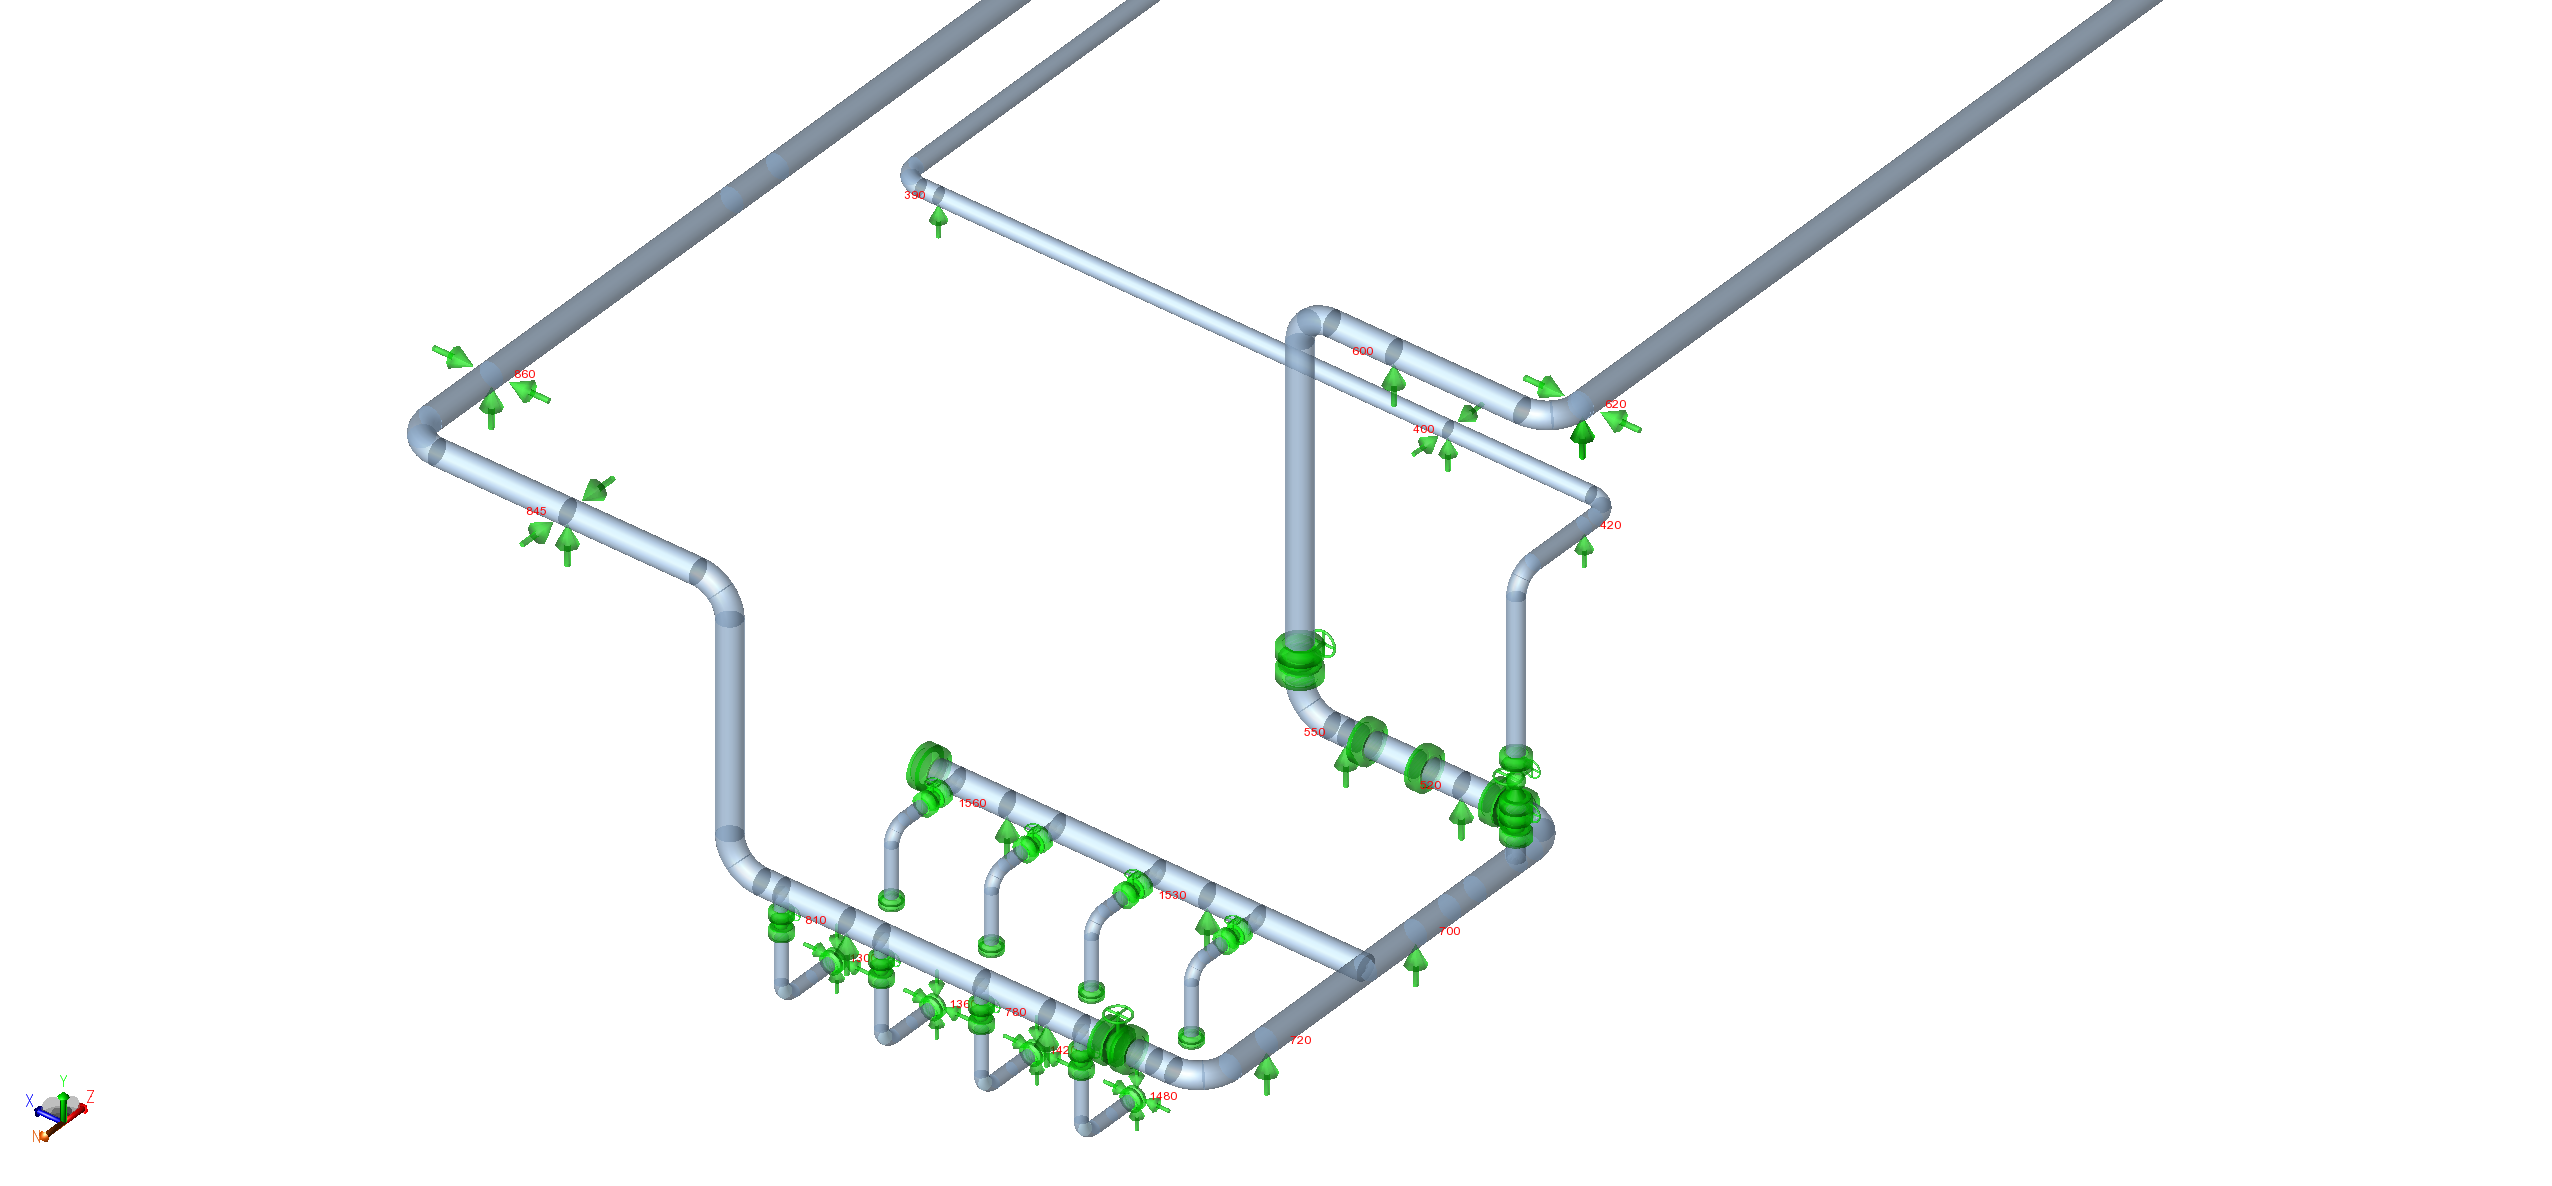
\includegraphics[width=0.85\textwidth]{assets/graf_nodos_soporte.png}
    \caption{Modelo de CAESAR II con los soportes y restricciones de la l\'{i}nea, vista 1 (job P2603-PR-SIM-023).}
    \label{fig:nodos-soporte}
\end{figure}

\begin{figure}[htbp]
    \centering
    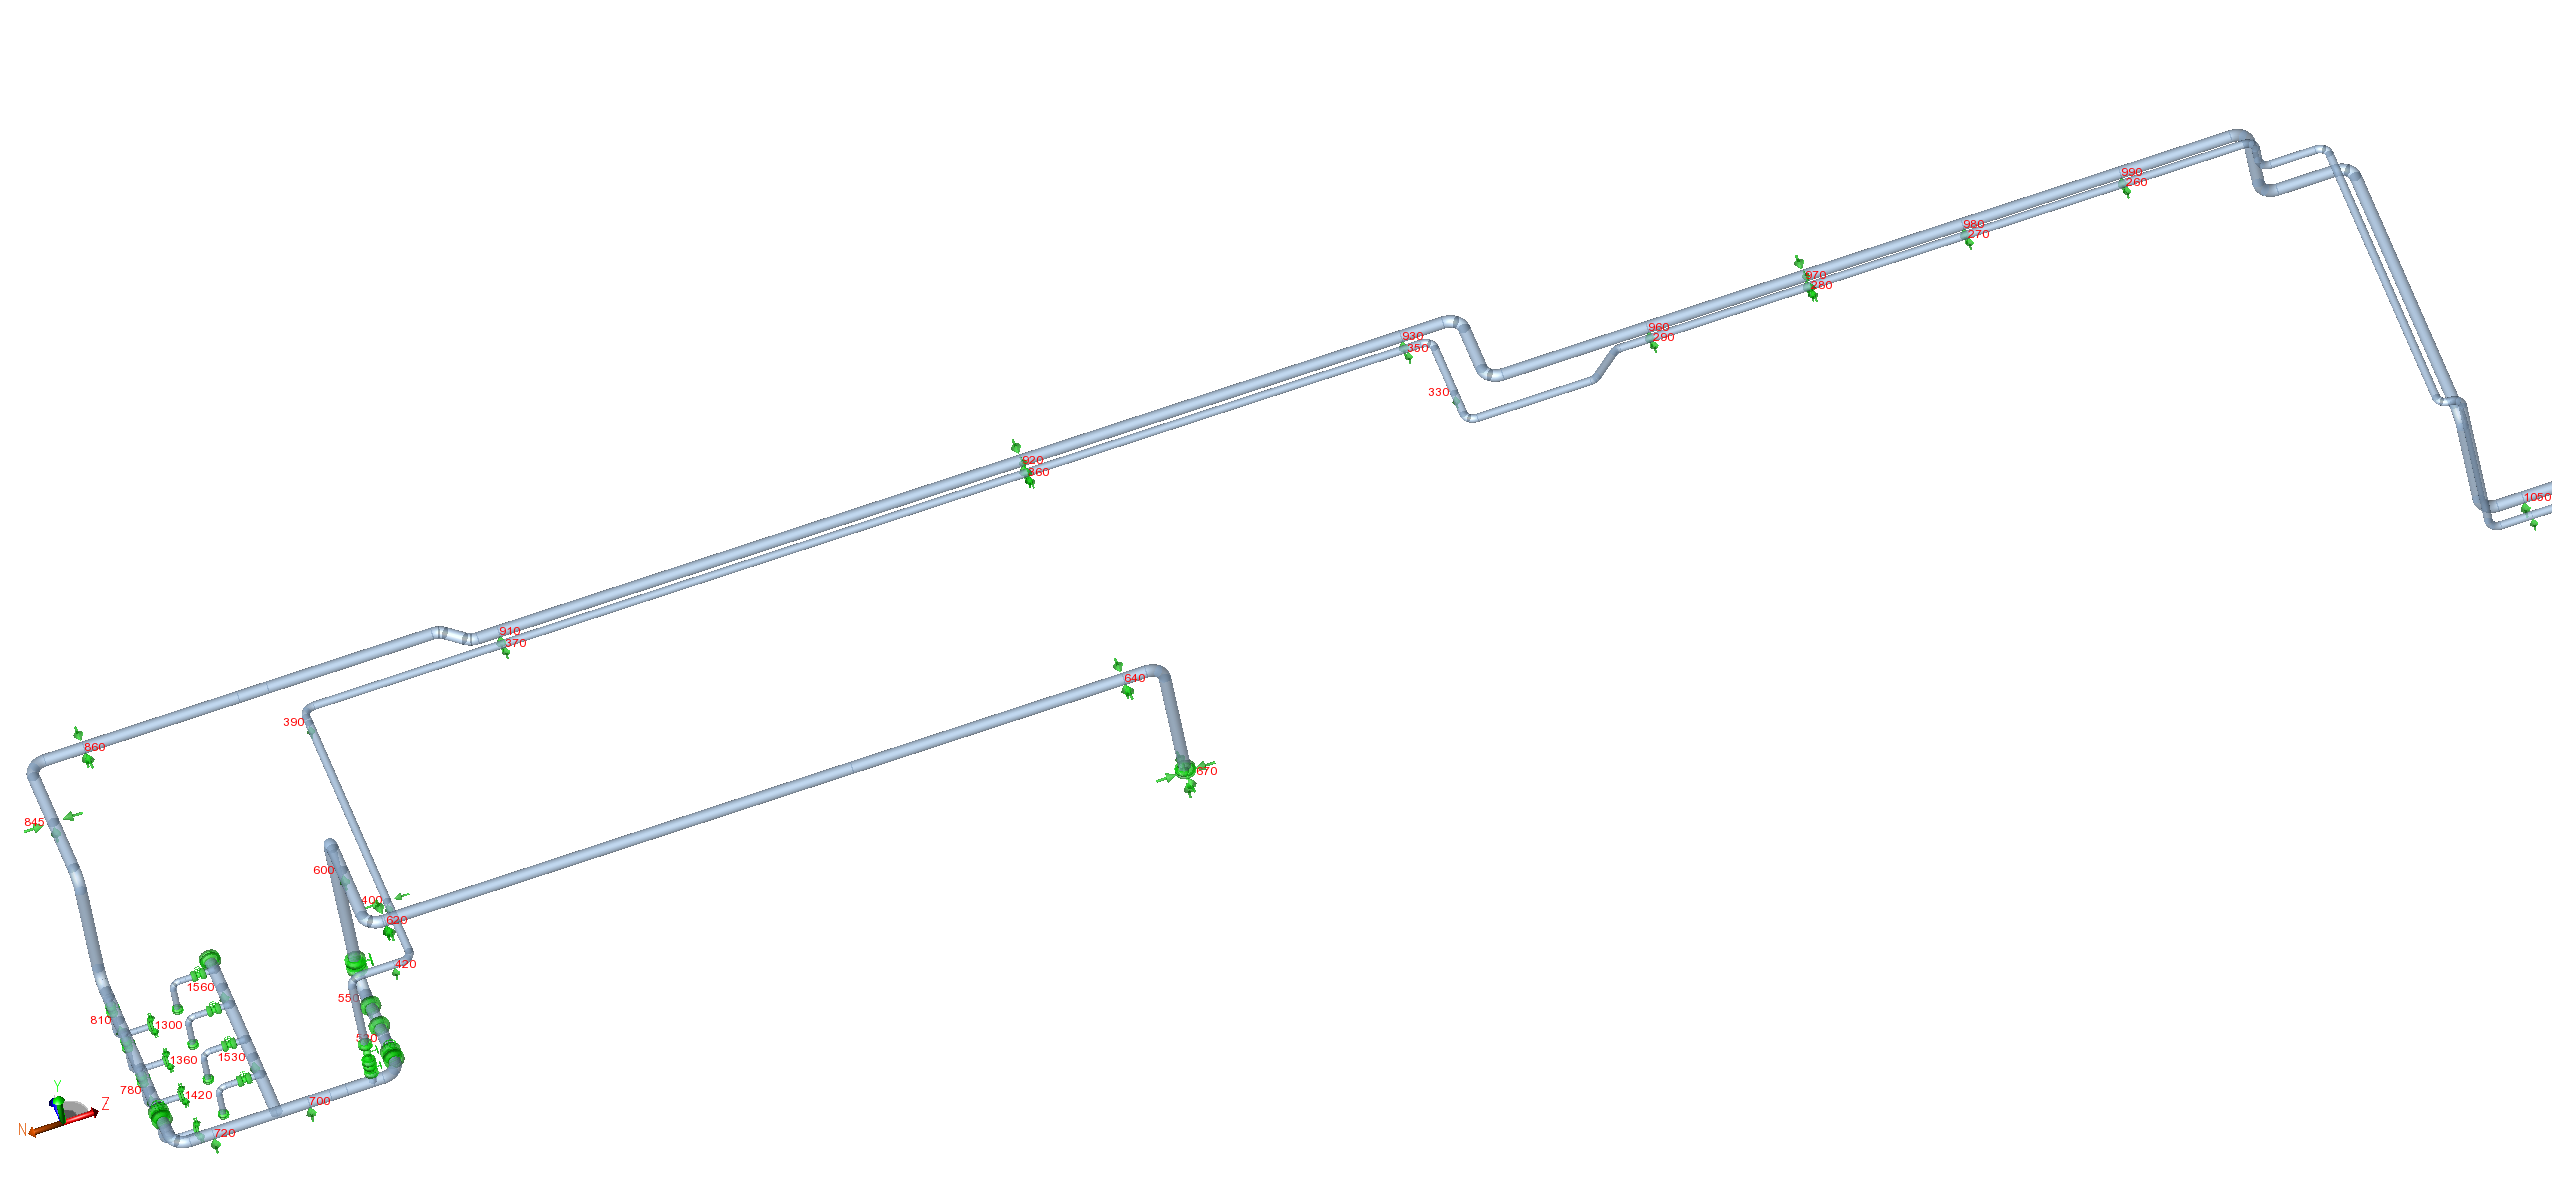
\includegraphics[width=0.85\textwidth]{assets/graf_nodos_soporte_2.png}
    \caption{Modelo de CAESAR II con los soportes y restricciones de la l\'{i}nea, vista 2 (job P2603-PR-SIM-023).}
    \label{fig:nodos-soporte-2}
\end{figure}

\begin{figure}[htbp]
    \centering
    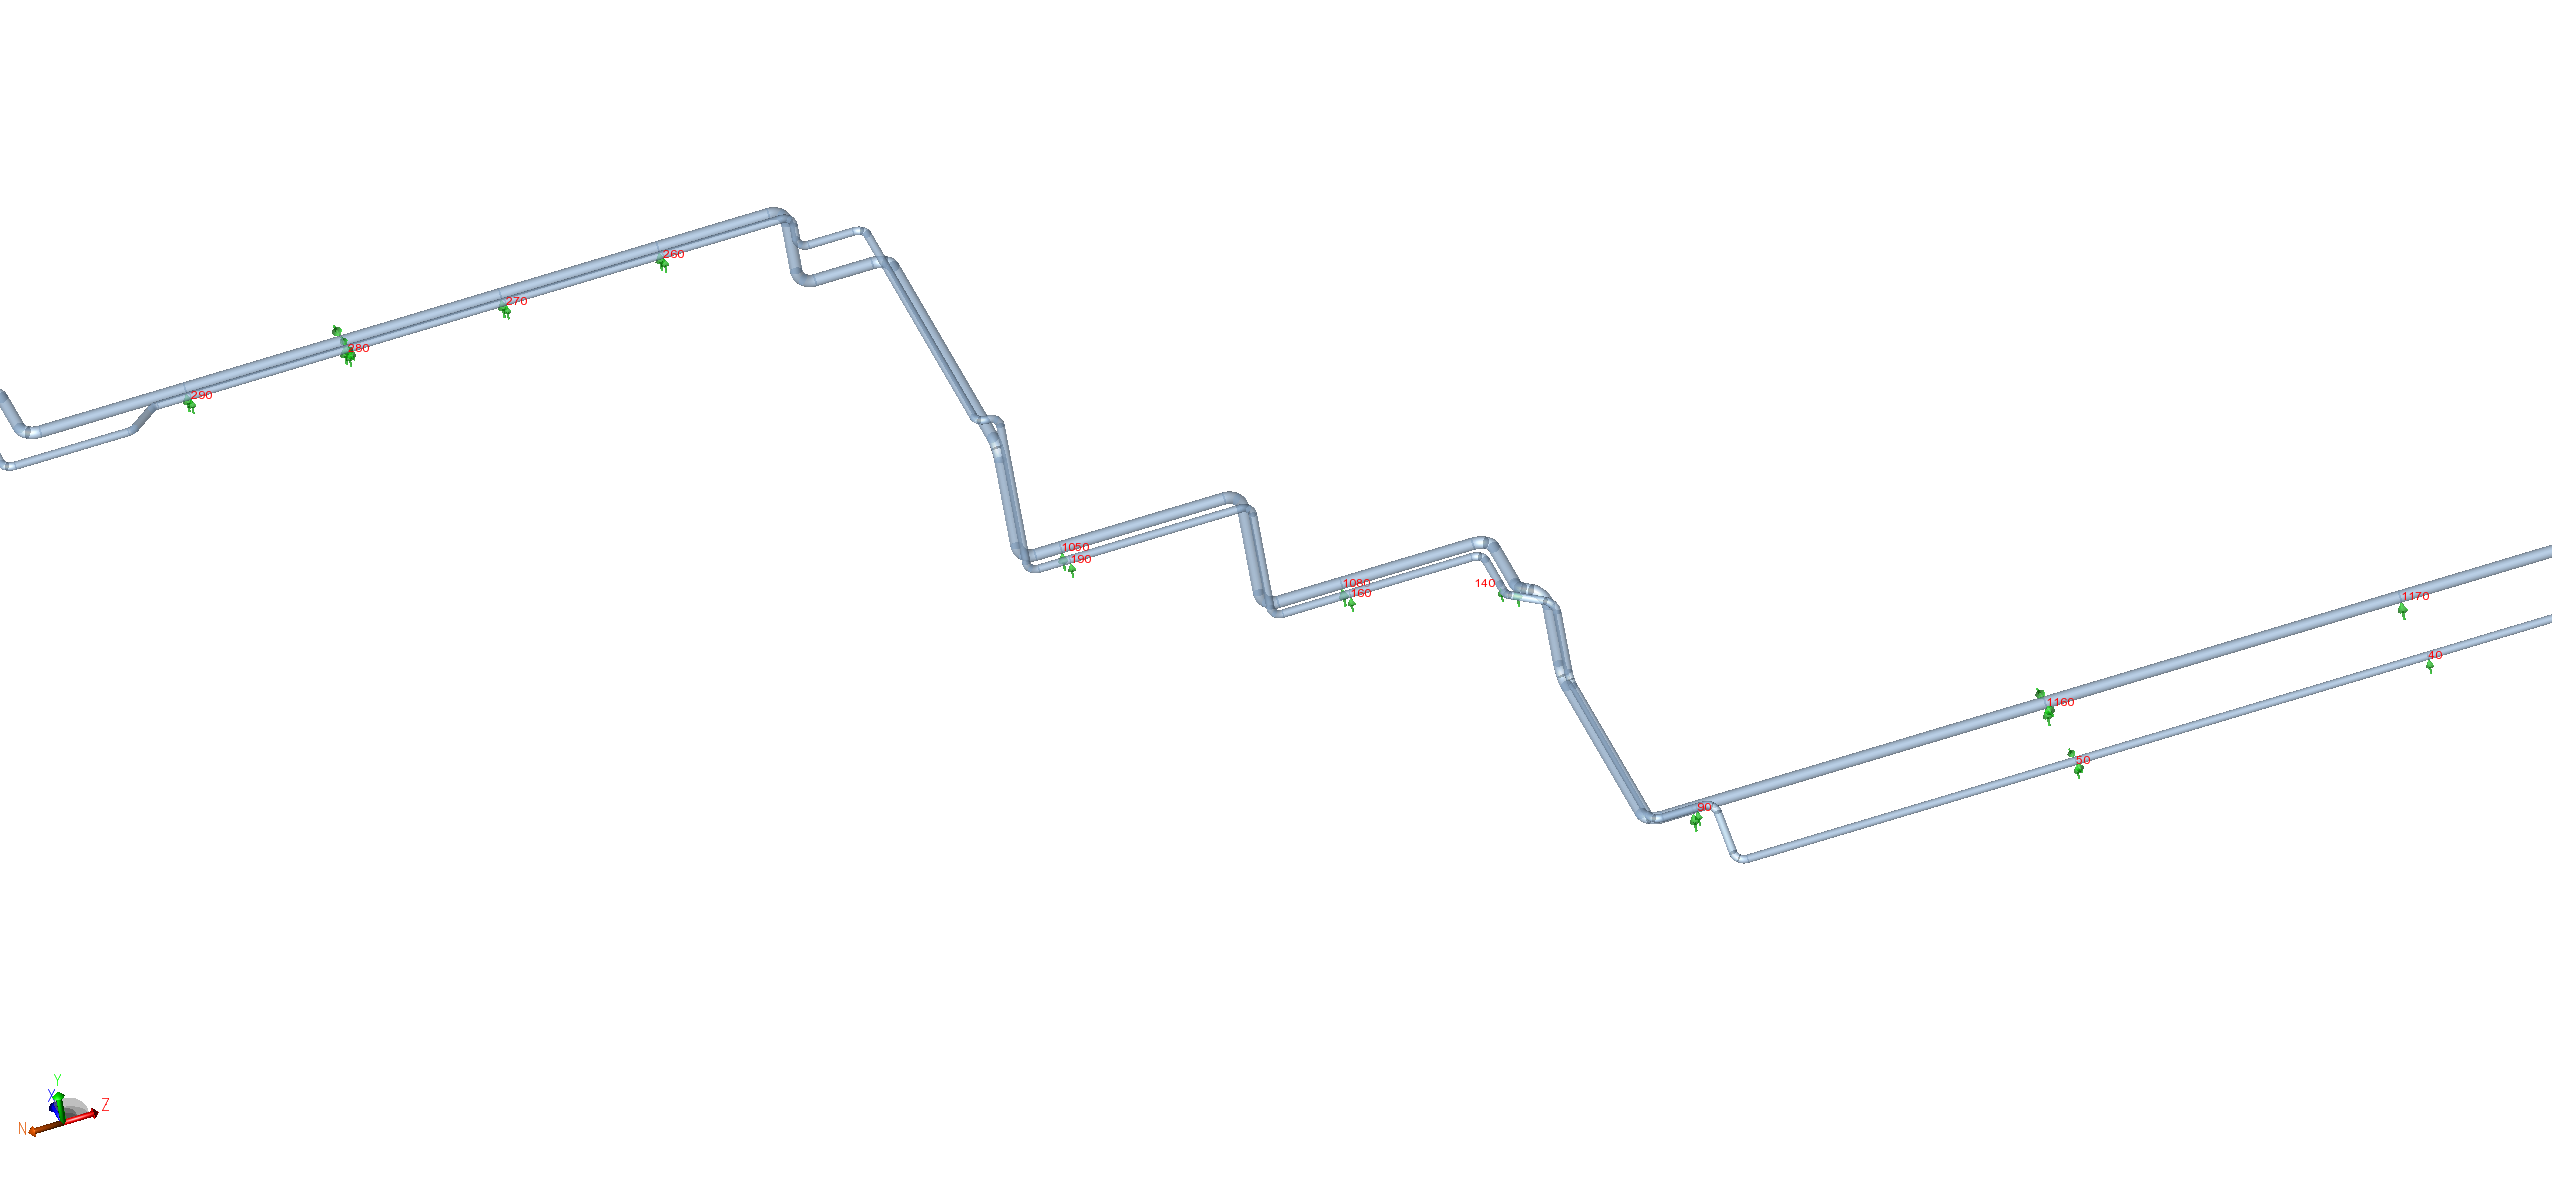
\includegraphics[width=0.85\textwidth]{assets/graf_nodos_soporte_3.png}
    \caption{Modelo de CAESAR II con los soportes y restricciones de la l\'{i}nea, vista 3 (job P2603-PR-SIM-023).}
    \label{fig:nodos-soporte-3}
\end{figure}

\begin{figure}[htbp]
    \centering
    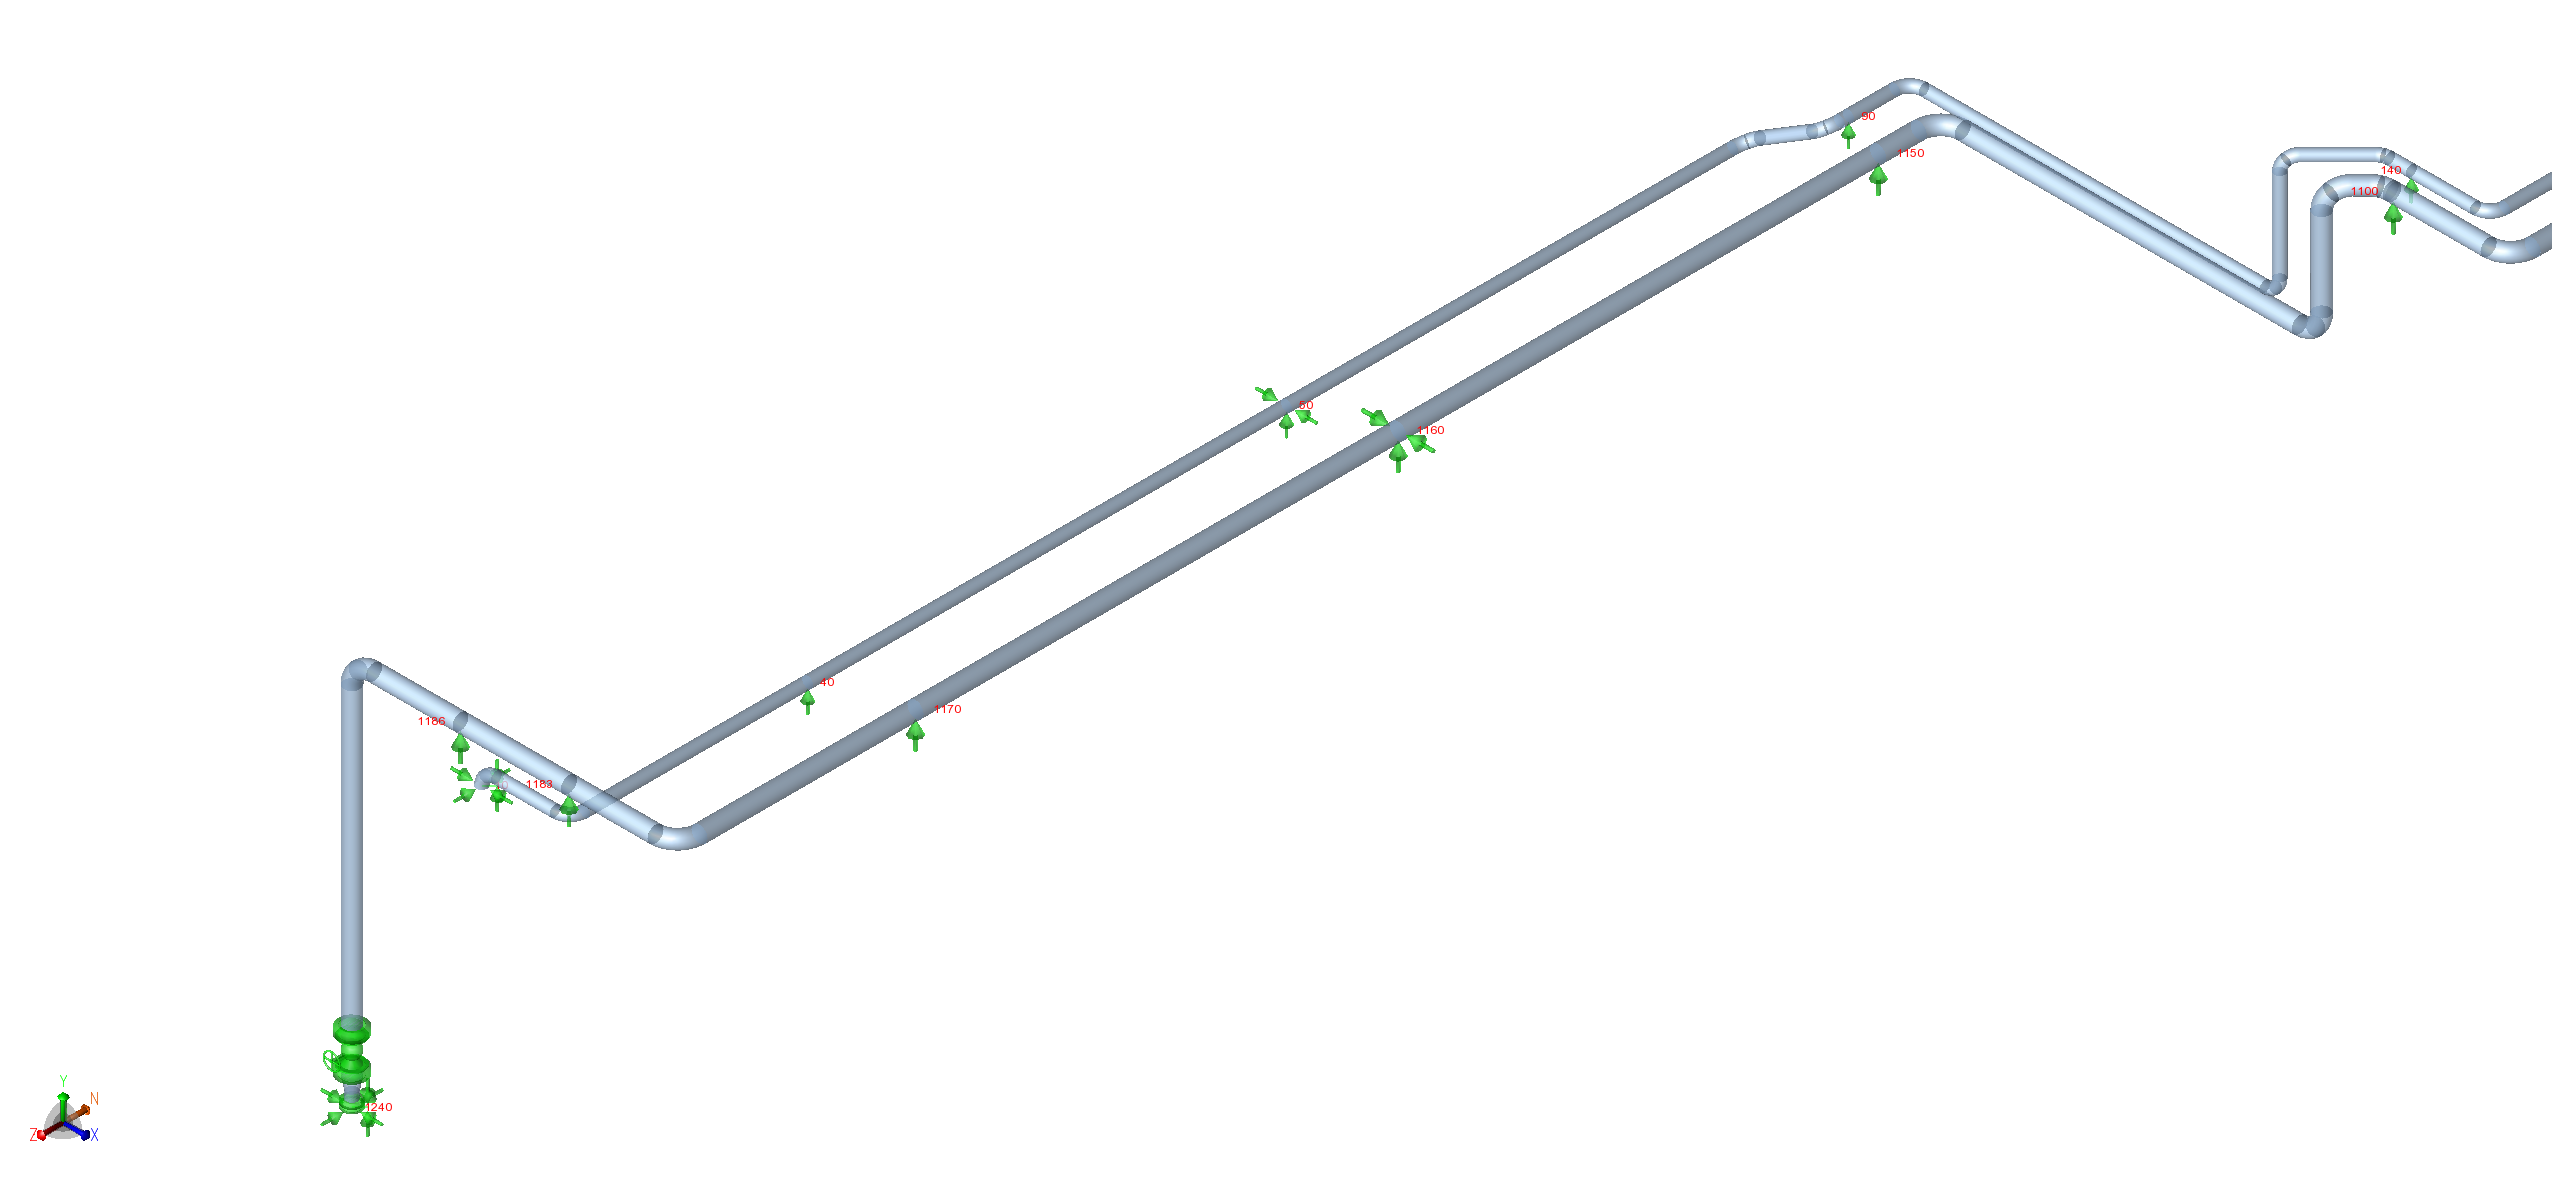
\includegraphics[width=0.85\textwidth]{assets/graf_nodos_soporte_4.png}
    \caption{Modelo de CAESAR II con los soportes y restricciones de la l\'{i}nea, vista 4 (job P2603-PR-SIM-023).}
    \label{fig:nodos-soporte-4}
\end{figure}

% ─────────────────────────────────────────────────────────────────────────────
\subsection{Isometrico de Referencia}

La Figura~\ref{fig:isometrico} presenta la vista del modelo 3D de dise\~{n}o de
la l\'{i}nea, correspondiente al isom\'{e}trico PCF119 empleado como fuente
geom\'{e}trica del modelo de esfuerzos.

\begin{figure}[htbp]
    \centering
    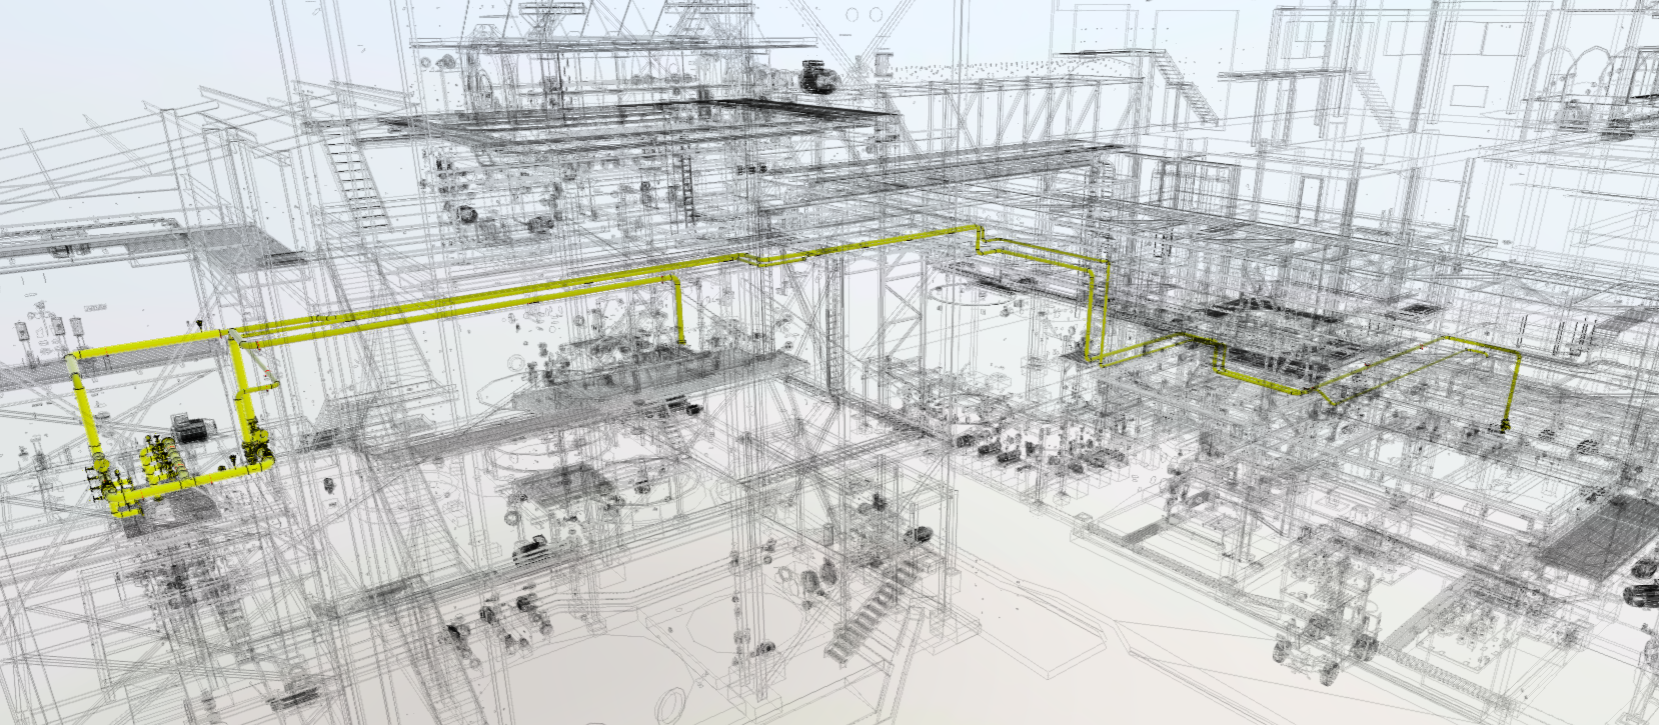
\includegraphics[width=0.95\textwidth]{assets/PCF119.png}
    \caption{Vista del modelo 3D de la l\'{i}nea de alimentaci\'{o}n a los limpiadores de arena (PCF119, AutoCAD Plant 3D 2027).}
    \label{fig:isometrico}
\end{figure}
